% Requires in the preamble:
% \usepackage{amsmath,amssymb}
% \usepackage{tikz,pgfplots}
% \pgfplotsset{compat=1.18}

\chapter{Shape, Extremes, and the Mean Value Theorem}
\label{chap:shape-extremes-mvt}

Chapter 5 gave us a working language for derivatives.  We learned how to
differentiate sums, products, quotients, compositions, inverse functions, and the
elementary functions.

That language is useful because a derivative is more than a formula.  It is
information about shape.

If

\[
f'(x)>0,
\]

then the graph wants to rise.  If

\[
f'(x)<0,
\]

then the graph wants to fall.  If

\[
f'(x)=0,
\]

then the graph has a horizontal tangent.  A horizontal tangent may mark a high
point, a low point, or only a momentary pause.

This chapter asks how far we can push that idea.

\[
\text{derivative information}
\quad\Longrightarrow\quad
\text{shape information}.
\]

The answer will lead to one of the central theorems of differential calculus: the
Mean Value Theorem.

\section{Increasing and decreasing functions}
\label{sec:increasing-decreasing-functions}

A speedometer does not only tell how fast a car is moving.  Its sign tells the
direction of motion.  Positive velocity means position is increasing.  Negative
velocity means position is decreasing.

The same idea works for any differentiable function.

\subsection{Reading motion from the sign of velocity}
\label{subsec:reading-motion-from-sign-velocity}

Suppose a particle moves along a line, and its position after \(t\) seconds is

\[
s(t)=t^3-6t^2+9t,
\qquad 0\le t\le 4.
\]

Its velocity is the derivative:

\[
v(t)=s'(t)=3t^2-12t+9.
\]

Factor:

\[
v(t)=3(t-1)(t-3).
\]

This factorization tells us the sign of the velocity.

\[
\begin{array}{c|c|c}
\text{time interval} & \text{sign of } v(t) & \text{motion} \\ \hline
0<t<1 & + & \text{position increases} \\
1<t<3 & - & \text{position decreases} \\
3<t<4 & + & \text{position increases}
\end{array}
\]

At

\[
t=1
\qquad\text{and}\qquad
t=3,
\]

the velocity is \(0\).  These are the moments when the particle changes direction.

\begin{figure}[h]
\centering
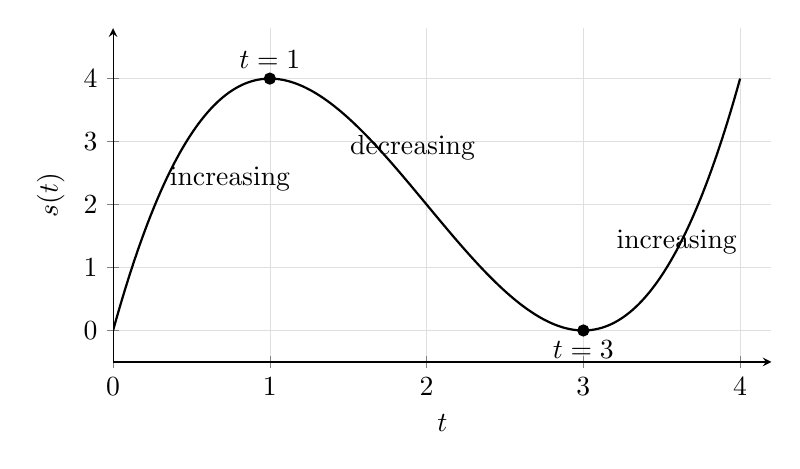
\begin{tikzpicture}
\begin{axis}[
    width=0.82\textwidth,
    height=0.48\textwidth,
    xmin=0, xmax=4.2,
    ymin=-0.5, ymax=4.8,
    axis lines=left,
    xlabel={\(t\)},
    ylabel={\(s(t)\)},
    xtick={0,1,2,3,4},
    ytick={0,1,2,3,4},
    grid=both,
    grid style={line width=.1pt, draw=gray!25},
]
\addplot[thick, domain=0:4, samples=200] {x^3-6*x^2+9*x};
\addplot[only marks, mark=*] coordinates {(1,4) (3,0)};
\node[anchor=south] at (axis cs:1,4) {\(t=1\)};
\node[anchor=north] at (axis cs:3,0) {\(t=3\)};
\node[anchor=west] at (axis cs:0.3,2.4) {increasing};
\node[anchor=west] at (axis cs:1.45,2.9) {decreasing};
\node[anchor=west] at (axis cs:3.15,1.4) {increasing};
\end{axis}
\end{tikzpicture}

\vspace{0.5em}

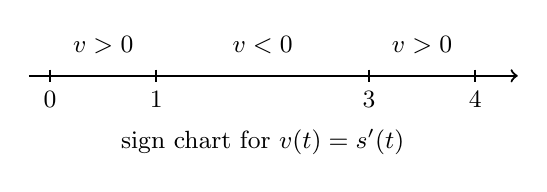
\begin{tikzpicture}[xscale=1.35, every node/.style={font=\small}]
  \draw[->, thick] (-0.2,0) -- (4.4,0);
  \foreach \x/\lab in {0/0,1/1,3/3,4/4} {
    \draw[thick] (\x,0.08) -- (\x,-0.08);
    \node[below] at (\x,-0.08) {\(\lab\)};
  }
  \node[above] at (0.5,0.15) {\(v>0\)};
  \node[above] at (2,0.15) {\(v<0\)};
  \node[above] at (3.5,0.15) {\(v>0\)};
  \node[below] at (2,-0.55) {sign chart for \(v(t)=s'(t)\)};
\end{tikzpicture}

\caption{The sign of velocity tells whether the position is increasing or decreasing.}
\label{fig:position-sign-chart}
\end{figure}

The graph confirms the algebra.  The position rises until \(t=1\), falls until
\(t=3\), and rises again.

The derivative has become a guide to the shape of the original function.

\subsection{Increasing and decreasing functions}
\label{subsec:increasing-decreasing-definitions}

The motion example suggests the general language.

\begin{quote}
\textbf{Increasing and decreasing.}
Let \(f\) be a function on an interval \(I\).

The function \(f\) is \emph{increasing} on \(I\) if, whenever

\[
x_1<x_2
\]

in \(I\), we have

\[
f(x_1)<f(x_2).
\]

The function \(f\) is \emph{decreasing} on \(I\) if, whenever

\[
x_1<x_2
\]

in \(I\), we have

\[
f(x_1)>f(x_2).
\]
\end{quote}

Increasing means that moving to the right on the input line moves upward on the
graph.  Decreasing means that moving to the right moves downward on the graph.

A function can increase on one interval and decrease on another.  The function

\[
s(t)=t^3-6t^2+9t
\]

is increasing on

\[
[0,1]
\]

and on

\[
[3,4],
\]

but decreasing on

\[
[1,3].
\]

The intervals matter.

\subsection{The first derivative sign rule}
\label{subsec:first-derivative-sign-rule}

The examples point to the rule we want.

\begin{quote}
\textbf{First derivative sign rule.}
Suppose \(f\) is continuous on an interval \(I\) and differentiable at the interior
points of \(I\).

If

\[
f'(x)>0
\]

throughout the interior of \(I\), then \(f\) is increasing on \(I\).

If

\[
f'(x)<0
\]

throughout the interior of \(I\), then \(f\) is decreasing on \(I\).
\end{quote}

This rule is one of the most useful tools in differential calculus.  Its proof will
come from the Mean Value Theorem in Section \ref{sec:rolle-mvt}.  For now, the
meaning is visible from local linear approximation:

\[
f(x+h)\approx f(x)+f'(x)h.
\]

When \(h>0\), moving to the right by a small amount, a positive \(f'(x)\) gives a
positive change in \(f\).  A negative \(f'(x)\) gives a negative change in \(f\).

The Mean Value Theorem will explain why this local information controls the
whole interval.

\subsection{First derivative sign charts}
\label{subsec:first-derivative-sign-charts}

A \emph{sign chart} turns derivative information into graph information.

Consider

\[
f(x)=x^3-3x.
\]

Then

\[
f'(x)=3x^2-3=3(x-1)(x+1).
\]

The derivative is zero at

\[
x=-1
\qquad\text{and}\qquad
x=1.
\]

These two numbers split the real line into three intervals:

\[
(-\infty,-1),
\qquad
(-1,1),
\qquad
(1,\infty).
\]

Now test the sign of \(f'\) on each interval.

\[
\begin{array}{c|c|c}
\text{interval} & \text{sign of } f'(x) & \text{behavior of } f \\ \hline
(-\infty,-1) & + & \text{increasing} \\
(-1,1) & - & \text{decreasing} \\
(1,\infty) & + & \text{increasing}
\end{array}
\]

So the graph rises, then falls, then rises again.

\begin{figure}[h]
\centering
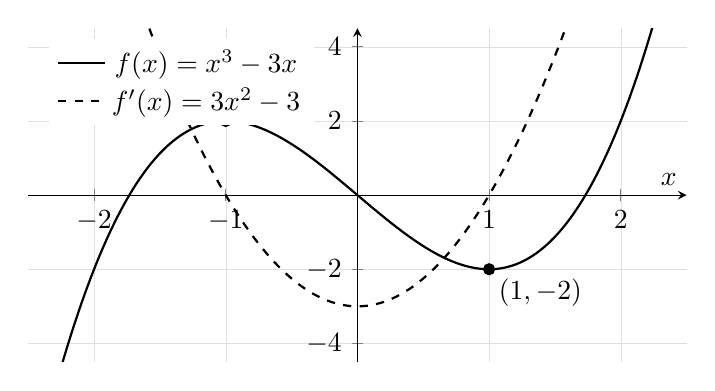
\begin{tikzpicture}
\begin{axis}[
    width=0.82\textwidth,
    height=0.48\textwidth,
    xmin=-2.5, xmax=2.5,
    ymin=-4.5, ymax=4.5,
    axis lines=middle,
    xlabel={\(x\)},
    ylabel={},
    xtick={-2,-1,0,1,2},
    ytick={-4,-2,0,2,4},
    grid=both,
    grid style={line width=.1pt, draw=gray!25},
    legend style={draw=none, at={(0.03,0.97)}, anchor=north west}
]
\addplot[thick, domain=-2.25:2.25, samples=200] {x^3-3*x};
\addlegendentry{\(f(x)=x^3-3x\)}
\addplot[thick, dashed, domain=-2.25:2.25, samples=200] {3*x^2-3};
\addlegendentry{\(f'(x)=3x^2-3\)}
\addplot[only marks, mark=*] coordinates {(-1,2) (1,-2)};
\node[anchor=south east] at (axis cs:-1,2) {\((-1,2)\)};
\node[anchor=north west] at (axis cs:1,-2) {\((1,-2)\)};
\end{axis}
\end{tikzpicture}

\vspace{0.5em}

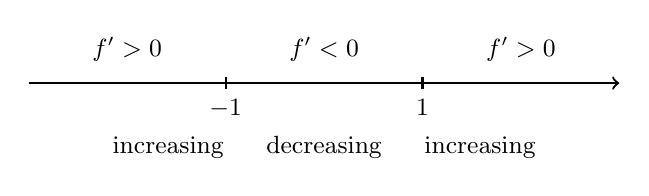
\begin{tikzpicture}[xscale=1.25, every node/.style={font=\small}]
  \draw[->, thick] (-3.0,0) -- (3.0,0);
  \draw[thick] (-1,0.08) -- (-1,-0.08);
  \draw[thick] (1,0.08) -- (1,-0.08);
  \node[below] at (-1,-0.08) {\(-1\)};
  \node[below] at (1,-0.08) {\(1\)};
  \node[above] at (-2,0.15) {\(f'>0\)};
  \node[above] at (0,0.15) {\(f'<0\)};
  \node[above] at (2,0.15) {\(f'>0\)};
  \node[below] at (0,-0.55) {increasing \(\quad\) decreasing \(\quad\) increasing};
\end{tikzpicture}

\caption{The derivative sign chart predicts the rise and fall of the original graph.}
\label{fig:first-derivative-sign-chart}
\end{figure}

The method has a simple rhythm.

\begin{quote}
\textbf{Making a first derivative sign chart.}

\[
\begin{array}{ll}
\text{1.} & \text{Compute } f'(x).\\
\text{2.} & \text{Find where } f'(x)=0 \text{ or where } f'(x) \text{ does not exist.}\\
\text{3.} & \text{Use those numbers to split the domain into intervals.}\\
\text{4.} & \text{Test the sign of } f'(x) \text{ on each interval.}\\
\text{5.} & \text{Translate } f'>0 \text{ into increasing, and } f'<0 \text{ into decreasing.}
\end{array}
\]
\end{quote}

The derivative does not need to be drawn.  The sign chart may contain all the
information we need.

\subsection{Critical numbers}
\label{subsec:critical-numbers}

The numbers where the derivative is zero or undefined deserve a name.

\begin{quote}
\textbf{Critical number.}
Let \(c\) be a number in the domain of \(f\).  We call \(c\) a \emph{critical number}
of \(f\) if

\[
f'(c)=0
\]

or if

\[
f'(c)
\]

does not exist.
\end{quote}

The phrase ``in the domain of \(f\)'' matters.  A function can only have a critical
number at an input where the function itself is defined.

For

\[
f(x)=x^3-3x,
\]

the critical numbers are

\[
-1
\qquad\text{and}\qquad
1.
\]

For

\[
g(x)=|x|,
\]

the number

\[
0
\]

is a critical number because \(g'(0)\) does not exist.  The graph has a corner there.

\begin{figure}[h]
\centering
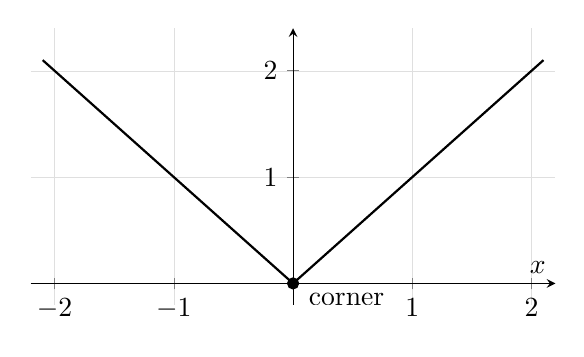
\begin{tikzpicture}
\begin{axis}[
    width=0.68\textwidth,
    height=0.42\textwidth,
    xmin=-2.2, xmax=2.2,
    ymin=-0.2, ymax=2.4,
    axis lines=middle,
    xlabel={\(x\)},
    ylabel={},
    xtick={-2,-1,0,1,2},
    ytick={0,1,2},
    grid=both,
    grid style={line width=.1pt, draw=gray!25},
]
\addplot[thick, domain=-2.1:0, samples=2] {-x};
\addplot[thick, domain=0:2.1, samples=2] {x};
\addplot[only marks, mark=*] coordinates {(0,0)};
\node[anchor=north west] at (axis cs:0.05,0) {corner};
\end{axis}
\end{tikzpicture}
\caption{For \(g(x)=|x|\), the derivative is undefined at \(0\).  So \(0\) is a critical number.}
\label{fig:absolute-value-critical}
\end{figure}

A critical number is a candidate for an important point on the graph.  It is not a
promise.

For example,

\[
h(x)=x^3
\]

has derivative

\[
h'(x)=3x^2.
\]

So

\[
h'(0)=0.
\]

The number \(0\) is critical.  But \(h(x)=x^3\) keeps increasing through \(0\).  It
does not turn around there.

\[
\boxed{
\text{Critical numbers are candidates, not conclusions.}
}
\]

The next section asks which critical numbers actually give high points or low points.

\section{Local and absolute extrema}
\label{sec:local-absolute-extrema}

The sign chart for \(x^3-3x\) showed a graph that rises, then falls, then rises.
At the point where rising changes to falling, the graph has a high point nearby.
At the point where falling changes to rising, the graph has a low point nearby.

Those points are called extrema.

\subsection{Local maximum and local minimum}
\label{subsec:local-max-local-min}

A high point nearby is not necessarily the highest point everywhere.  A mountain
can have many peaks.  A small peak is still a peak if the graph is lower on both
sides nearby.

\begin{quote}
\textbf{Local extrema.}
A function \(f\) has a \emph{local maximum} at \(c\) if

\[
f(c)\ge f(x)
\]

for all \(x\) sufficiently close to \(c\).

A function \(f\) has a \emph{local minimum} at \(c\) if

\[
f(c)\le f(x)
\]

for all \(x\) sufficiently close to \(c\).
\end{quote}

The phrase ``sufficiently close'' means that we only compare \(f(c)\) with nearby
values of the function.  Local extrema are neighborhood ideas.

Now compare this with the global idea.

\begin{quote}
\textbf{Absolute extrema.}
A function \(f\) has an \emph{absolute maximum} at \(c\) on a set \(D\) if

\[
f(c)\ge f(x)
\]

for every \(x\in D\).

A function \(f\) has an \emph{absolute minimum} at \(c\) on a set \(D\) if

\[
f(c)\le f(x)
\]

for every \(x\in D\).
\end{quote}

Absolute extrema compare against the whole domain under discussion.  Local extrema
compare only nearby.

\paragraph{Example.}
Let

\[
f(x)=x^3-6x^2+9x+2,
\qquad \frac12\le x\le 5.
\]

Then

\[
f'(x)=3x^2-12x+9=3(x-1)(x-3).
\]

The derivative changes from positive to negative at \(x=1\), so \(x=1\) is a local
maximum.  The derivative changes from negative to positive at \(x=3\), so \(x=3\)
is a local minimum.

But the absolute maximum on the interval occurs at the endpoint \(x=5\).  A
local maximum does not have to be the absolute maximum.

\begin{figure}[h]
\centering
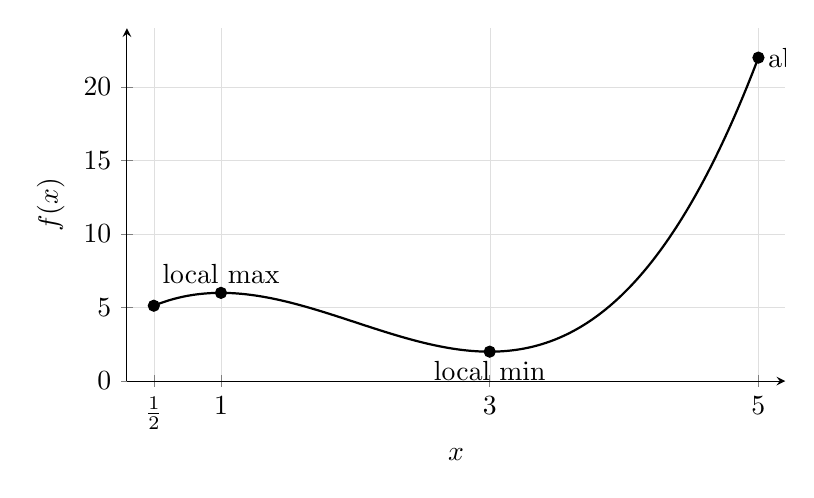
\begin{tikzpicture}
\begin{axis}[
    width=0.82\textwidth,
    height=0.50\textwidth,
    xmin=0.3, xmax=5.2,
    ymin=0, ymax=24,
    axis lines=left,
    xlabel={\(x\)},
    ylabel={\(f(x)\)},
    xtick={0.5,1,3,5},
    xticklabels={\(\frac12\),\(1\),\(3\),\(5\)},
    ytick={0,5,10,15,20},
    grid=both,
    grid style={line width=.1pt, draw=gray!25},
]
\addplot[thick, domain=0.5:5, samples=200] {x^3-6*x^2+9*x+2};
\addplot[only marks, mark=*] coordinates {(0.5,5.125) (1,6) (3,2) (5,22)};
\node[anchor=south] at (axis cs:1,6) {local max};
\node[anchor=north] at (axis cs:3,2) {local min};
\node[anchor=west] at (axis cs:5,22) {absolute max};
\end{axis}
\end{tikzpicture}
\caption{A local maximum may not be the absolute maximum.  Endpoints must be checked.}
\label{fig:local-vs-absolute-extrema}
\end{figure}

\subsection{Fermat's theorem}
\label{subsec:fermats-theorem-extrema}

At a smooth local maximum, the tangent line is horizontal.  The graph rises into
the point and falls away from it.  The left-side slopes and right-side slopes force
the tangent slope to be \(0\).

At a smooth local minimum, the same thing happens upside down.

\begin{quote}
\textbf{Fermat's theorem.}
Suppose \(f\) has a local maximum or local minimum at an interior point \(c\).  If
\(f\) is differentiable at \(c\), then

\[
\boxed{f'(c)=0.}
\]
\end{quote}

\paragraph{Proof.}
We prove the local maximum case.  The local minimum case is similar.

Assume \(f\) has a local maximum at \(c\).  Then for all \(x\) close enough to \(c\),

\[
f(x)\le f(c).
\]

For \(h>0\) small enough,

\[
f(c+h)-f(c)\le 0.
\]

Dividing by the positive number \(h\), we get

\[
\frac{f(c+h)-f(c)}{h}\le 0.
\]

So the right-hand difference quotients are less than or equal to \(0\).

For \(h<0\) small enough, the numerator still satisfies

\[
f(c+h)-f(c)\le 0,
\]

but now the denominator \(h\) is negative.  Dividing by a negative number reverses
the inequality:

\[
\frac{f(c+h)-f(c)}{h}\ge 0.
\]

So the left-hand difference quotients are greater than or equal to \(0\).

If \(f'(c)\) exists, then the left-hand and right-hand limits of these quotients must
agree.  The only number that can be both

\[
\le 0
\]

and

\[
\ge 0
\]

is \(0\).  Therefore

\[
f'(c)=0.
\]

\subsection{Why Fermat's hypotheses matter}
\label{subsec:fermat-hypotheses-matter}

Fermat's theorem is short, but every condition is doing work.

\paragraph{Endpoint warning.}
Let

\[
f(x)=x
\]

on the interval

\[
[0,1].
\]

The function has an absolute minimum at \(x=0\) and an absolute maximum at \(x=1\).
But

\[
f'(x)=1
\]

everywhere.

There is no contradiction.  Fermat's theorem applies to interior points, not endpoints.
At an endpoint, the graph can be highest or lowest simply because the interval stops.

\paragraph{Corner warning.}
Let

\[
f(x)=|x|.
\]

This function has a local minimum at \(x=0\).  But

\[
f'(0)
\]

does not exist.  Again, Fermat's theorem is not contradicted.  The theorem says that
if the local extremum occurs at a differentiable interior point, then the derivative
is \(0\).

Corners can have extrema without horizontal tangents.

\paragraph{Critical number warning.}
The converse of Fermat's theorem is false.

Fermat's theorem says:

\[
\text{differentiable local extremum}
\quad\Longrightarrow\quad
f'(c)=0.
\]

It does not say:

\[
f'(c)=0
\quad\Longrightarrow\quad
\text{local extremum}.
\]

For example,

\[
f(x)=x^3
\]

has

\[
f'(x)=3x^2,
\]

so

\[
f'(0)=0.
\]

But \(x^3\) is increasing through \(0\).  It has neither a local maximum nor a local
minimum there.

\[
\boxed{
\text{Every differentiable interior extremum is critical, but not every critical number is an extremum.}
}
\]

\subsection{The first derivative test}
\label{subsec:first-derivative-test}

A critical number becomes more meaningful when we look at the sign of \(f'\) on
both sides.

\begin{quote}
\textbf{First derivative test.}
Suppose \(c\) is a critical number of \(f\), and \(f\) is continuous at \(c\).

\[
\begin{array}{c|c|c}
\text{sign of } f' \text{ before } c & \text{sign of } f' \text{ after } c & \text{conclusion} \\ \hline
+ & - & \text{local maximum at } c \\
- & + & \text{local minimum at } c \\
+ & + & \text{no local extremum forced} \\
- & - & \text{no local extremum forced}
\end{array}
\]
\end{quote}

The reason is simple.  If the function increases before \(c\) and decreases after
\(c\), then \(c\) is a high point nearby.  If it decreases before \(c\) and increases
after \(c\), then \(c\) is a low point nearby.

This test depends on the first derivative sign rule, whose full proof comes from the
Mean Value Theorem.  The picture is already clear; the next theorem will make it
secure.

\paragraph{Example.}
For

\[
f(x)=x^3-3x,
\]

we found

\[
f'(x)=3(x-1)(x+1).
\]

The sign chart is

\[
\begin{array}{c|ccc}
x & (-\infty,-1) & (-1,1) & (1,\infty) \\ \hline
f'(x) & + & - & +
\end{array}
\]

So \(f\) has a local maximum at

\[
x=-1
\]

and a local minimum at

\[
x=1.
\]

The values are

\[
f(-1)=2,
\qquad
f(1)=-2.
\]

\subsection{Absolute extrema and the closed interval method}
\label{subsec:closed-interval-method}

Local extrema are nearby comparisons.  Absolute extrema are whole-domain
comparisons.  To find them, we need a guarantee that they exist.

The guarantee comes from continuity on a closed, bounded interval.

\begin{quote}
\textbf{Extreme Value Theorem.}
If \(f\) is continuous on a closed interval \([a,b]\), then \(f\) has an absolute
maximum and an absolute minimum on \([a,b]\).
\end{quote}

This theorem is a deep fact about the real line.  It rests on the idea that the real
line has no gaps.  For now, its meaning is more important than its proof:

\[
\text{a continuous graph on a closed finite interval cannot escape its highest and lowest values.}
\]

The hypotheses matter.

\paragraph{Open interval warning.}
The function

\[
f(x)=x
\]

on

\[
(0,1)
\]

has no absolute maximum and no absolute minimum.  Its values get close to \(1\),
but never equal \(1\).  They get close to \(0\), but never equal \(0\).

The interval is not closed.

\paragraph{Unbounded interval warning.}
The function

\[
f(x)=x
\]

on

\[
[0,\infty)
\]

has an absolute minimum at \(0\), but no absolute maximum.

The interval is not bounded.

\paragraph{Continuity warning.}
Define

\[
f(x)=
\begin{cases}
x, & 0\le x<1,\\
0, & x=1.
\end{cases}
\]

on \([0,1]\).  This function has no absolute maximum.  The values approach \(1\),
but the function never reaches \(1\).  At the endpoint, it jumps down to \(0\).

The interval is closed and bounded, but the function is not continuous.

\subsection{The closed interval method}
\label{subsec:closed-interval-method-procedure}

Fermat's theorem tells us where an interior extremum can occur.  The Extreme Value
Theorem tells us that absolute extrema exist on a closed interval.  Together they
give a practical method.

\begin{quote}
\textbf{Closed interval method.}
To find the absolute maximum and minimum of a continuous function \(f\) on
\([a,b]\):

\[
\begin{array}{ll}
\text{1.} & \text{Find all critical numbers of } f \text{ in } (a,b).\\
\text{2.} & \text{Evaluate } f \text{ at those critical numbers.}\\
\text{3.} & \text{Evaluate } f(a) \text{ and } f(b).\\
\text{4.} & \text{Compare the values.  The largest is the absolute maximum value.}\\
          & \text{The smallest is the absolute minimum value.}
\end{array}
\]
\end{quote}

Endpoints are included because Fermat's theorem does not apply there.  An endpoint
can be the best or worst value simply because the graph stops.

\paragraph{Example.}
Find the absolute maximum and minimum of

\[
f(x)=x^3-6x^2+9x+2
\]

on

\[
\left[\frac12,5\right].
\]

First compute the derivative:

\[
f'(x)=3x^2-12x+9.
\]

Factor:

\[
f'(x)=3(x-1)(x-3).
\]

So the critical numbers inside the interval are

\[
x=1
\qquad\text{and}\qquad
x=3.
\]

Now evaluate \(f\) at the critical numbers and endpoints.

\[
\begin{array}{c|c}
x & f(x) \\ \hline
\frac12 & \frac{41}{8} \\[3pt]
1 & 6 \\[3pt]
3 & 2 \\[3pt]
5 & 22
\end{array}
\]

The smallest value is

\[
2,
\]

which occurs at

\[
x=3.
\]

The largest value is

\[
22,
\]

which occurs at

\[
x=5.
\]

Therefore \(f\) has absolute minimum value \(2\) at \(x=3\), and absolute maximum
value \(22\) at \(x=5\).

Notice what happened.  The local maximum at \(x=1\) is not the absolute maximum.
The endpoint \(x=5\) wins.

\[
\boxed{
\text{On a closed interval, always check endpoints.}
}
\]

\subsection{Where this points}
\label{subsec:extrema-hook-mvt}

We have used the derivative to read the shape of a function:

\[
f'>0 \quad\Rightarrow\quad \text{increasing},
\]

\[
f'<0 \quad\Rightarrow\quad \text{decreasing},
\]

and

\[
\text{smooth local extremum} \quad\Rightarrow\quad f'=0.
\]

Fermat's theorem was proved directly from the derivative definition.  But the first
derivative sign rule still needs its real proof.

The missing idea is surprisingly simple.  If a car's average velocity over a trip is
\(50\) miles per hour, then at some instant its speed should have been \(50\) miles
per hour.  If a smooth graph starts and ends at the same height, then somewhere in
between it should have a horizontal tangent.

That idea is Rolle's Theorem, and just beyond it is the Mean Value Theorem.
\section{Rolle's Theorem and the Mean Value Theorem}
\label{sec:rolle-mvt}

Section \ref{sec:local-absolute-extrema} gave us two tools.

First, a continuous function on a closed interval reaches its absolute maximum and
minimum.  Second, a differentiable local extremum at an interior point must have
derivative \(0\).

Those two facts now combine into a theorem about motion.

Suppose a car is at mile marker \(10\) at noon and mile marker \(160\) at
\(3{:}00\).  Its average velocity is

\[
\frac{160-10}{3-0}=50
\]

miles per hour.

The car may have driven slowly at first and quickly later.  It may have stopped for
a short time.  But if its position changed continuously, and if its velocity existed
during the trip, then at some instant the speedometer must have read

\[
50\text{ miles per hour}.
\]

That is the meaning of the Mean Value Theorem.

\subsection{A road trip with average velocity}
\label{subsec:road-trip-average-velocity}

Let \(s(t)\) be the position of the car, measured in miles, \(t\) hours after noon.
The average velocity from \(t=a\) to \(t=b\) is

\[
\frac{s(b)-s(a)}{b-a}.
\]

The instantaneous velocity is

\[
s'(t).
\]

The claim is that, under the right hypotheses, some instantaneous velocity equals the
average velocity:

\[
s'(c)=\frac{s(b)-s(a)}{b-a}
\]

for some time \(c\) between \(a\) and \(b\).

Geometrically, the average velocity is the slope of a secant line.  The instantaneous
velocity is the slope of a tangent line.  So the claim becomes:

\[
\text{some tangent line is parallel to the secant line.}
\]

\begin{figure}[h]
\centering
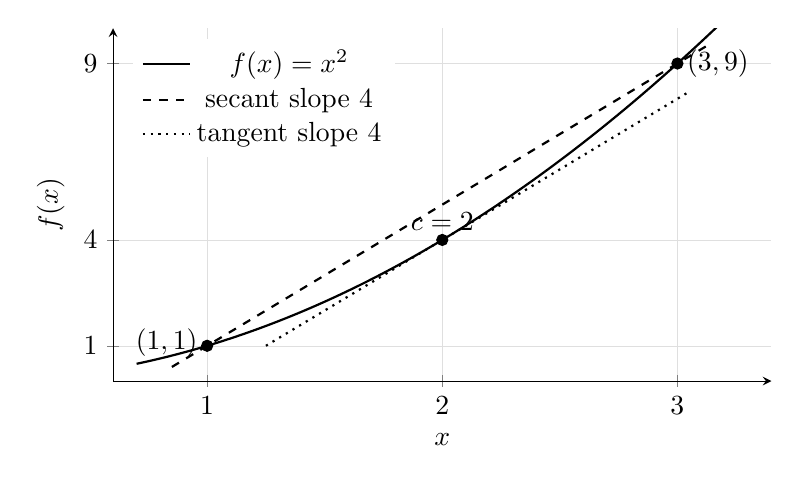
\begin{tikzpicture}
\begin{axis}[
    width=0.82\textwidth,
    height=0.50\textwidth,
    xmin=0.6, xmax=3.4,
    ymin=0, ymax=10,
    axis lines=left,
    xlabel={\(x\)},
    ylabel={\(f(x)\)},
    xtick={1,2,3},
    ytick={1,4,9},
    grid=both,
    grid style={line width=.1pt, draw=gray!25},
    legend style={draw=none, at={(0.03,0.97)}, anchor=north west}
]
\addplot[thick, domain=0.7:3.25, samples=200] {x^2};
\addlegendentry{\(f(x)=x^2\)}

% secant line through (1,1) and (3,9): y=4x-3
\addplot[thick, dashed, domain=0.85:3.15, samples=2] {4*x-3};
\addlegendentry{secant slope \(4\)}

% tangent at x=2: y=4x-4
\addplot[thick, dotted, domain=1.25:3.05, samples=2] {4*x-4};
\addlegendentry{tangent slope \(4\)}

\addplot[only marks, mark=*] coordinates {(1,1) (2,4) (3,9)};
\node[anchor=east] at (axis cs:1,1.1) {\((1,1)\)};
\node[anchor=west] at (axis cs:3,9) {\((3,9)\)};
\node[anchor=south] at (axis cs:2,4) {\(c=2\)};
\end{axis}
\end{tikzpicture}
\caption{For \(f(x)=x^2\) on \([1,3]\), the secant slope is \(4\).  The tangent slope at \(x=2\) is also \(4\).}
\label{fig:mvt-parabola}
\end{figure}

For the function in Figure \ref{fig:mvt-parabola},

\[
f(x)=x^2,
\qquad 1\le x\le 3.
\]

The average rate of change is

\[
\frac{f(3)-f(1)}{3-1}
=
\frac{9-1}{2}
=
4.
\]

Since

\[
f'(x)=2x,
\]

we solve

\[
2c=4
\]

and get

\[
c=2.
\]

So the tangent at \(x=2\) is parallel to the secant line from \(x=1\) to \(x=3\).

Before proving the full theorem, we prove its flat special case.

\subsection{Rolle's Theorem}
\label{subsec:rolles-theorem}

Suppose a graph starts and ends at the same height.  If it is smooth in between,
then somewhere in between it must have a horizontal tangent.

For example, let

\[
f(x)=x^2-4x+3
\]

on \([1,3]\).  Then

\[
f(1)=0,
\qquad
f(3)=0.
\]

The derivative is

\[
f'(x)=2x-4.
\]

So

\[
f'(2)=0.
\]

The graph starts at height \(0\), ends at height \(0\), and turns at \(x=2\).

\begin{figure}[h]
\centering
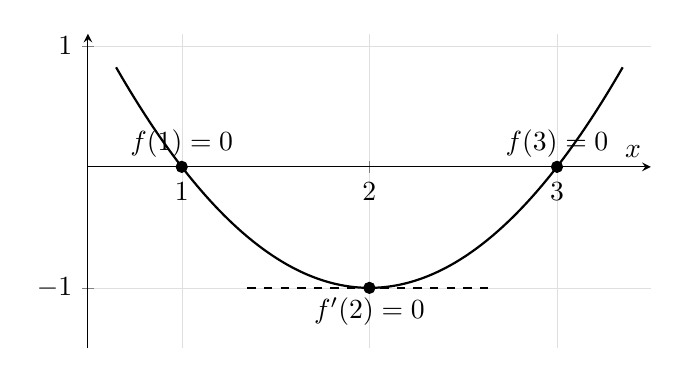
\begin{tikzpicture}
\begin{axis}[
    width=0.72\textwidth,
    height=0.46\textwidth,
    xmin=0.5, xmax=3.5,
    ymin=-1.5, ymax=1.1,
    axis lines=middle,
    xlabel={\(x\)},
    ylabel={},
    xtick={1,2,3},
    ytick={-1,0,1},
    grid=both,
    grid style={line width=.1pt, draw=gray!25}
]
\addplot[thick, domain=0.65:3.35, samples=200] {x^2-4*x+3};
\addplot[thick, dashed, domain=1.35:2.65, samples=2] {-1};
\addplot[only marks, mark=*] coordinates {(1,0) (2,-1) (3,0)};
\node[anchor=south] at (axis cs:1,0) {\(f(1)=0\)};
\node[anchor=south] at (axis cs:3,0) {\(f(3)=0\)};
\node[anchor=north] at (axis cs:2,-1) {\(f'(2)=0\)};
\end{axis}
\end{tikzpicture}
\caption{Rolle's Theorem says that equal endpoint heights force at least one horizontal tangent inside.}
\label{fig:rolles-theorem-example}
\end{figure}

\begin{quote}
\textbf{Rolle's Theorem.}
Suppose \(f\) is continuous on \([a,b]\) and differentiable on \((a,b)\).  If

\[
f(a)=f(b),
\]

then there is at least one number \(c\) in \((a,b)\) such that

\[
\boxed{f'(c)=0.}
\]
\end{quote}

\paragraph{Proof.}
Because \(f\) is continuous on the closed interval \([a,b]\), the Extreme Value
Theorem says that \(f\) reaches an absolute maximum and an absolute minimum on
\([a,b]\).

If \(f\) is constant on \([a,b]\), then

\[
f'(c)=0
\]

for every \(c\in(a,b)\), and we are done.

Now suppose \(f\) is not constant.  Since

\[
f(a)=f(b),
\]

the absolute maximum or the absolute minimum must occur at an interior point.  Call
that point \(c\).

At this interior point, \(f\) has a local extremum.  Since \(f\) is differentiable at
\(c\), Fermat's theorem gives

\[
f'(c)=0.
\]

This proves Rolle's Theorem.

\subsection{Why Rolle's hypotheses matter}
\label{subsec:rolle-hypotheses-matter}

Each hypothesis prevents a different kind of escape.

\paragraph{Continuity warning.}
Define

\[
f(x)=
\begin{cases}
x, & 0\le x<1,\\
0, & x=1.
\end{cases}
\]

on \([0,1]\).  Then

\[
f(0)=0,
\qquad
f(1)=0.
\]

The function is differentiable on \((0,1)\), and

\[
f'(x)=1
\]

there.  There is no point \(c\in(0,1)\) with \(f'(c)=0\).

The problem is that \(f\) is not continuous on \([0,1]\).  The graph climbs toward
\(1\), then jumps down at the endpoint.

\paragraph{Differentiability warning.}
Let

\[
f(x)=|x|
\]

on \([-1,1]\).  Then

\[
f(-1)=1,
\qquad
f(1)=1.
\]

The function is continuous, but it is not differentiable at \(0\).  On the left,

\[
f'(x)=-1,
\]

and on the right,

\[
f'(x)=1.
\]

There is no interior point where the derivative exists and equals \(0\).  The graph
turns at a corner instead of a horizontal tangent.

\paragraph{Endpoint-height warning.}
Let

\[
f(x)=x
\]

on \([0,1]\).  This function is continuous and differentiable, but

\[
f(0)\neq f(1).
\]

There is no reason to expect a horizontal tangent.  Indeed,

\[
f'(x)=1
\]

everywhere.

\subsection{The Mean Value Theorem}
\label{subsec:mean-value-theorem}

Rolle's Theorem handles the flat case, when the endpoint heights are equal.  The
Mean Value Theorem handles every secant line.

\begin{quote}
\textbf{Mean Value Theorem.}
Suppose \(f\) is continuous on \([a,b]\) and differentiable on \((a,b)\).  Then there is
at least one number \(c\) in \((a,b)\) such that

\[
\boxed{
f'(c)=\frac{f(b)-f(a)}{b-a}.
}
\]
\end{quote}

The conclusion can also be written as

\[
f(b)-f(a)=f'(c)(b-a).
\]

This says:

\[
\text{total change}
=
\text{instantaneous rate at some hidden point}
\cdot
\text{input change}.
\]

The point \(c\) may be hard to find.  The theorem promises that it exists.

\paragraph{Example.}
Let

\[
f(x)=\sqrt{x}
\]

on \([1,4]\).  The average rate of change is

\[
\frac{f(4)-f(1)}{4-1}
=
\frac{2-1}{3}
=
\frac13.
\]

Since

\[
f'(x)=\frac1{2\sqrt{x}},
\]

the Mean Value Theorem says that some \(c\in(1,4)\) satisfies

\[
\frac1{2\sqrt{c}}=\frac13.
\]

Solving,

\[
2\sqrt{c}=3,
\qquad
\sqrt{c}=\frac32,
\qquad
c=\frac94.
\]

So at \(x=\frac94\), the tangent slope equals the secant slope from \(x=1\) to
\(x=4\).

\paragraph{Proof of the Mean Value Theorem.}
Let

\[
m=\frac{f(b)-f(a)}{b-a}.
\]

This is the slope of the secant line through \((a,f(a))\) and \((b,f(b))\).

The equation of that secant line is

\[
L(x)=f(a)+m(x-a).
\]

Now measure the vertical difference between the graph and the secant line:

\[
F(x)=f(x)-L(x).
\]

At the left endpoint,

\[
F(a)=f(a)-L(a)=f(a)-f(a)=0.
\]

At the right endpoint,

\[
L(b)=f(a)+m(b-a)
=
f(a)+\frac{f(b)-f(a)}{b-a}(b-a)
=
f(b),
\]

so

\[
F(b)=f(b)-L(b)=0.
\]

Thus

\[
F(a)=F(b).
\]

The function \(F\) is continuous on \([a,b]\) and differentiable on \((a,b)\), because
\(f\) and \(L\) have those properties.  Rolle's Theorem applies to \(F\).  Therefore
there is some \(c\in(a,b)\) such that

\[
F'(c)=0.
\]

But

\[
F'(x)=f'(x)-L'(x)=f'(x)-m.
\]

So

\[
0=F'(c)=f'(c)-m.
\]

Therefore

\[
f'(c)=m=\frac{f(b)-f(a)}{b-a}.
\]

This proves the Mean Value Theorem.

\subsection{Why the Mean Value Theorem hypotheses matter}
\label{subsec:mvt-hypotheses-matter}

The Mean Value Theorem has the same hypotheses as Rolle's Theorem, and for the
same reasons.

\paragraph{Continuity warning.}
Define

\[
f(x)=
\begin{cases}
x, & 0\le x<1,\\
0, & x=1.
\end{cases}
\]

on \([0,1]\).  Then

\[
\frac{f(1)-f(0)}{1-0}=0.
\]

But on the open interval \((0,1)\),

\[
f'(x)=1.
\]

There is no point \(c\in(0,1)\) where

\[
f'(c)=0.
\]

The Mean Value Theorem fails because the function is not continuous on the closed
interval.

\paragraph{Differentiability warning.}
Let

\[
f(x)=|x|
\]

on \([-1,1]\).  The average rate of change is

\[
\frac{f(1)-f(-1)}{1-(-1)}
=
\frac{1-1}{2}
=
0.
\]

But \(f'(x)=-1\) for \(x<0\), \(f'(x)=1\) for \(x>0\), and \(f'(0)\) does not exist.
There is no point where the derivative exists and equals \(0\).

The graph has a corner.  The theorem requires differentiability on the whole open
interval.

\subsection{Consequences of the Mean Value Theorem}
\label{subsec:mvt-consequences}

The Mean Value Theorem turns information about derivatives into information about
functions.  That is why it is so useful.

\begin{quote}
\textbf{Constant derivative theorem.}
If \(f'(x)=0\) for every \(x\) in an interval \(I\), then \(f\) is constant on \(I\).
\end{quote}

\paragraph{Proof.}
Choose any two numbers \(x_1<x_2\) in \(I\).  On the interval \([x_1,x_2]\), the
Mean Value Theorem gives some \(c\in(x_1,x_2)\) such that

\[
\frac{f(x_2)-f(x_1)}{x_2-x_1}=f'(c).
\]

But \(f'(c)=0\), so

\[
\frac{f(x_2)-f(x_1)}{x_2-x_1}=0.
\]

Since \(x_2-x_1\neq0\), this gives

\[
f(x_2)-f(x_1)=0,
\]

or

\[
f(x_2)=f(x_1).
\]

Any two values of the function are equal.  So \(f\) is constant on \(I\).

\begin{quote}
\textbf{Equal derivatives theorem.}
If

\[
f'(x)=g'(x)
\]

for every \(x\) in an interval \(I\), then \(f\) and \(g\) differ by a constant on \(I\).
That is,

\[
f(x)=g(x)+C
\]

for some constant \(C\).
\end{quote}

\paragraph{Proof.}
Let

\[
h(x)=f(x)-g(x).
\]

Then

\[
h'(x)=f'(x)-g'(x)=0.
\]

By the constant derivative theorem, \(h\) is constant on \(I\).  So

\[
f(x)-g(x)=C,
\]

which means

\[
f(x)=g(x)+C.
\]

This result will become important when we reverse differentiation.  If two functions
have the same derivative, they are not completely different.  They differ only by a
vertical shift.

\subsection{The first derivative sign rule, proved}
\label{subsec:first-derivative-sign-rule-proof}

Section \ref{subsec:first-derivative-sign-rule} used the first derivative sign rule.
Now we can prove it.

\begin{quote}
\textbf{First derivative sign rule.}
Suppose \(f\) is continuous on an interval \(I\) and differentiable at the interior
points of \(I\).

If

\[
f'(x)>0
\]

throughout the interior of \(I\), then \(f\) is increasing on \(I\).

If

\[
f'(x)<0
\]

throughout the interior of \(I\), then \(f\) is decreasing on \(I\).
\end{quote}

\paragraph{Proof.}
Choose two numbers \(x_1<x_2\) in \(I\).  By the Mean Value Theorem, there is a
number \(c\in(x_1,x_2)\) such that

\[
\frac{f(x_2)-f(x_1)}{x_2-x_1}=f'(c).
\]

If \(f'(x)>0\) throughout the interval, then

\[
f'(c)>0.
\]

Since

\[
x_2-x_1>0,
\]

we get

\[
f(x_2)-f(x_1)>0.
\]

Thus

\[
f(x_2)>f(x_1).
\]

So \(f\) is increasing.

The decreasing case is the same argument with \(f'(c)<0\), which gives

\[
f(x_2)-f(x_1)<0.
\]

Thus

\[
f(x_2)<f(x_1),
\]

so \(f\) is decreasing.

\subsection{A useful bound from derivatives}
\label{subsec:mvt-derivative-bound}

The Mean Value Theorem also turns a bound on the derivative into a bound on total
change.

Suppose

\[
|f'(x)|\le M
\]

for all \(x\in[a,b]\).  Then the Mean Value Theorem gives

\[
f(b)-f(a)=f'(c)(b-a)
\]

for some \(c\in(a,b)\).  Taking absolute values,

\[
|f(b)-f(a)|
=
|f'(c)|\,|b-a|
\le
M|b-a|.
\]

So

\[
\boxed{
|f(b)-f(a)|\le M|b-a|.
}
\]

This says that if the derivative is never large, then the function cannot change too
fast.  A bound on local change controls global change.

That idea will return when we estimate errors.

\subsection{Where this points}
\label{subsec:mvt-hook-concavity}

The Mean Value Theorem explains why the sign of \(f'\) controls increasing and
decreasing behavior.  It also explains why a zero derivative on an interval forces a
function to be constant.

But there is more shape left to read.

Two graphs can both be increasing and still look very different.  One can rise faster
and faster.  Another can rise more and more slowly.  The first derivative tells us
whether the graph rises or falls.  The next question asks whether the first derivative
itself is increasing or decreasing.

That is the second derivative.

\section{Concavity and second derivatives}
\label{sec:concavity-second-derivatives}

The first derivative tells whether a function is rising or falling.  It does not tell the
whole shape.

A car can move forward while speeding up.  It can also move forward while slowing
down.  In both cases the velocity is positive, but the motion feels different.

Graphs have the same distinction.  A graph can be increasing while bending upward,
or increasing while bending downward.  The second derivative measures that bending.

\subsection{Velocity changing: acceleration}
\label{subsec:velocity-changing-acceleration}

Let

\[
s(t)=t^2.
\]

Then

\[
v(t)=s'(t)=2t,
\]

and

\[
a(t)=v'(t)=s''(t)=2.
\]

The velocity is increasing.  The object is speeding up.  The graph of \(s(t)\) bends
upward.

Now let

\[
r(t)=6t-t^2
\]

on \(0\le t\le 3\).  Then

\[
r'(t)=6-2t.
\]

This velocity is positive on \(0<t<3\), so the position is still increasing.  But the
velocity is decreasing, because

\[
r''(t)=-2.
\]

The object is moving forward while slowing down.  The graph bends downward.

\begin{figure}[h]
\centering
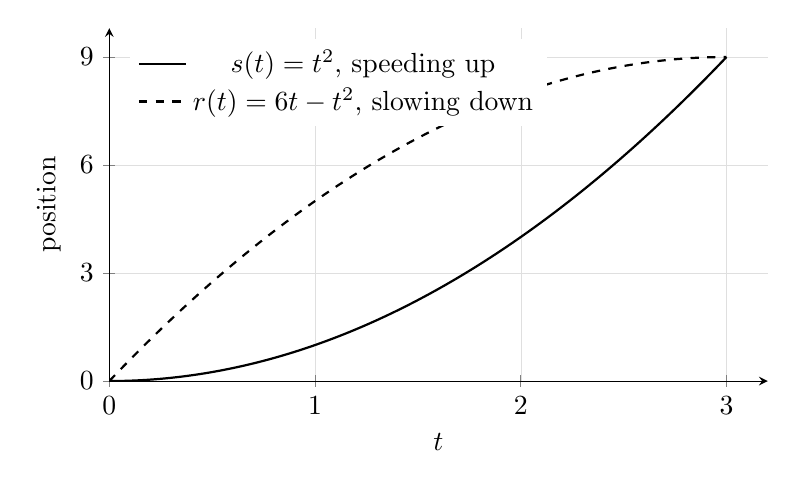
\begin{tikzpicture}
\begin{axis}[
    width=0.82\textwidth,
    height=0.50\textwidth,
    xmin=0, xmax=3.2,
    ymin=0, ymax=9.8,
    axis lines=left,
    xlabel={\(t\)},
    ylabel={position},
    xtick={0,1,2,3},
    ytick={0,3,6,9},
    grid=both,
    grid style={line width=.1pt, draw=gray!25},
    legend style={draw=none, at={(0.03,0.97)}, anchor=north west}
]
\addplot[thick, domain=0:3, samples=200] {x^2};
\addlegendentry{\(s(t)=t^2\), speeding up}

\addplot[thick, dashed, domain=0:3, samples=200] {6*x-x^2};
\addlegendentry{\(r(t)=6t-t^2\), slowing down}
\end{axis}
\end{tikzpicture}
\caption{Both positions increase on the interval, but one bends upward and the other bends downward.}
\label{fig:increasing-different-concavity}
\end{figure}

\begin{quote}
\textbf{Second derivative.}
If \(f'\) is differentiable, then the derivative of \(f'\) is called the second derivative
of \(f\):

\[
\boxed{
f''(x)=\frac{d}{dx}\bigl(f'(x)\bigr).
}
\]

In motion, if \(s(t)\) is position, then

\[
s'(t)=v(t)
\]

is velocity, and

\[
s''(t)=v'(t)=a(t)
\]

is acceleration.
\end{quote}

The units also tell the story.  If \(s(t)\) is measured in meters and \(t\) in seconds,
then

\[
s'(t)
\]

has units

\[
\frac{\text{meters}}{\text{second}},
\]

and

\[
s''(t)
\]

has units

\[
\frac{\text{meters}}{\text{second}^2}.
\]

Acceleration measures how fast velocity changes.

\subsection{Concave up and concave down}
\label{subsec:concave-up-down}

The word \emph{concavity} describes the direction a graph bends.

If the slopes are increasing as we move left to right, the graph is \emph{concave up}.
It bends like a cup.

If the slopes are decreasing as we move left to right, the graph is \emph{concave down}.
It bends like a cap.

\begin{quote}
\textbf{Concavity.}
Suppose \(f\) is differentiable on an interval \(I\).

The function \(f\) is \emph{concave up} on \(I\) if \(f'\) is increasing on \(I\).

The function \(f\) is \emph{concave down} on \(I\) if \(f'\) is decreasing on \(I\).
\end{quote}

This definition says that concavity is really a statement about how the tangent slopes
change.

\[
\text{concave up}
\quad\Longleftrightarrow\quad
\text{slopes increase},
\]

\[
\text{concave down}
\quad\Longleftrightarrow\quad
\text{slopes decrease}.
\]

Because the second derivative is the derivative of \(f'\), the first derivative sign rule
applied to \(f'\) gives the main test.

\begin{quote}
\textbf{Second derivative sign rule.}
Suppose \(f''\) exists on an interval \(I\).

If

\[
f''(x)>0
\]

on \(I\), then \(f\) is concave up on \(I\).

If

\[
f''(x)<0
\]

on \(I\), then \(f\) is concave down on \(I\).
\end{quote}

The reason is direct.  If \(f''>0\), then \(f'\) is increasing.  If \(f''<0\), then
\(f'\) is decreasing.

\begin{figure}[h]
\centering
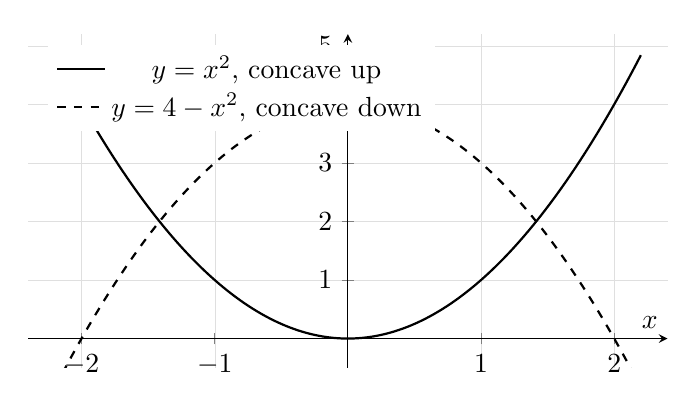
\begin{tikzpicture}
\begin{axis}[
    width=0.80\textwidth,
    height=0.48\textwidth,
    xmin=-2.4, xmax=2.4,
    ymin=-0.5, ymax=5.2,
    axis lines=middle,
    xlabel={\(x\)},
    ylabel={},
    xtick={-2,-1,0,1,2},
    ytick={0,1,2,3,4,5},
    grid=both,
    grid style={line width=.1pt, draw=gray!25},
    legend style={draw=none, at={(0.03,0.97)}, anchor=north west}
]
\addplot[thick, domain=-2.2:2.2, samples=200] {x^2};
\addlegendentry{\(y=x^2\), concave up}

\addplot[thick, dashed, domain=-2.2:2.2, samples=200] {4-x^2};
\addlegendentry{\(y=4-x^2\), concave down}
\end{axis}
\end{tikzpicture}
\caption{Concave up means slopes increase.  Concave down means slopes decrease.}
\label{fig:concave-up-down-basic}
\end{figure}

\subsection{A sign chart for the second derivative}
\label{subsec:second-derivative-sign-chart}

Consider again

\[
f(x)=x^3-3x.
\]

Then

\[
f'(x)=3x^2-3,
\]

and

\[
f''(x)=6x.
\]

The second derivative is negative when \(x<0\) and positive when \(x>0\).

\[
\begin{array}{c|c|c}
\text{interval} & \text{sign of } f''(x) & \text{concavity of } f \\ \hline
(-\infty,0) & - & \text{concave down} \\
(0,\infty) & + & \text{concave up}
\end{array}
\]

The graph bends downward to the left of \(0\), and upward to the right of \(0\).

\begin{figure}[h]
\centering
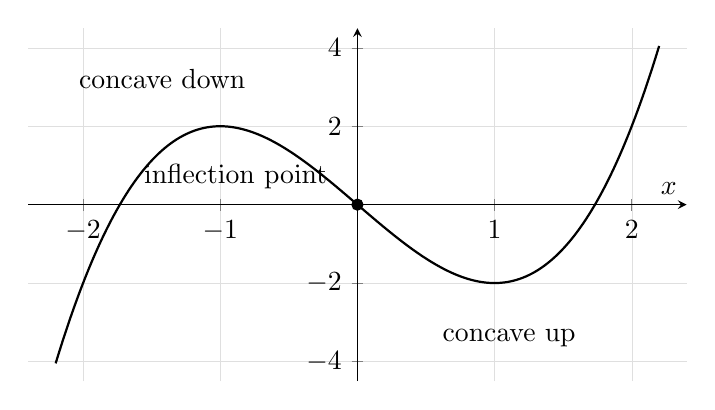
\begin{tikzpicture}
\begin{axis}[
    width=0.82\textwidth,
    height=0.50\textwidth,
    xmin=-2.4, xmax=2.4,
    ymin=-4.5, ymax=4.5,
    axis lines=middle,
    xlabel={\(x\)},
    ylabel={},
    xtick={-2,-1,0,1,2},
    ytick={-4,-2,0,2,4},
    grid=both,
    grid style={line width=.1pt, draw=gray!25}
]
\addplot[thick, domain=-2.2:2.2, samples=200] {x^3-3*x};
\draw[dashed] (axis cs:0,-4.2) -- (axis cs:0,4.2);
\addplot[only marks, mark=*] coordinates {(0,0)};
\node[anchor=south east] at (axis cs:-0.15,0.15) {inflection point};
\node[anchor=west] at (axis cs:-2.1,3.2) {concave down};
\node[anchor=west] at (axis cs:0.55,-3.4) {concave up};
\end{axis}
\end{tikzpicture}

\vspace{0.5em}

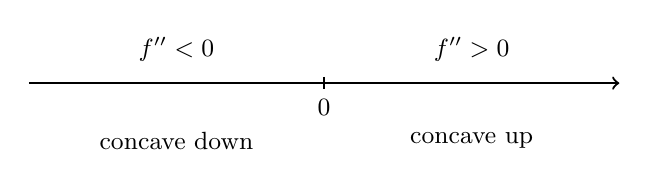
\begin{tikzpicture}[xscale=1.25, every node/.style={font=\small}]
  \draw[->, thick] (-3.0,0) -- (3.0,0);
  \draw[thick] (0,0.08) -- (0,-0.08);
  \node[below] at (0,-0.08) {\(0\)};
  \node[above] at (-1.5,0.15) {\(f''<0\)};
  \node[above] at (1.5,0.15) {\(f''>0\)};
  \node[below] at (-1.5,-0.50) {concave down};
  \node[below] at (1.5,-0.50) {concave up};
\end{tikzpicture}

\caption{The sign of \(f''\) gives the concavity of \(f\).}
\label{fig:cubic-concavity-chart}
\end{figure}

This example also shows a new kind of point: the graph changes concavity at
\(x=0\).

\subsection{Inflection points}
\label{subsec:inflection-points}

A point where the concavity changes is called an inflection point.

\begin{quote}
\textbf{Inflection point.}
A point \((c,f(c))\) on the graph of \(f\) is an \emph{inflection point} if the concavity
of \(f\) changes at \(c\).
\end{quote}

The number \(c\) is often found by looking for places where

\[
f''(c)=0
\]

or where

\[
f''(c)
\]

does not exist.  But these are only candidates.  The concavity must actually change.

\paragraph{Example: an inflection point.}
For

\[
f(x)=x^3,
\]

we have

\[
f'(x)=3x^2,
\qquad
f''(x)=6x.
\]

The second derivative changes from negative to positive at \(0\).  Therefore
\((0,0)\) is an inflection point.

\paragraph{Example: a false candidate.}
For

\[
g(x)=x^4,
\]

we have

\[
g'(x)=4x^3,
\qquad
g''(x)=12x^2.
\]

At \(x=0\),

\[
g''(0)=0.
\]

But

\[
g''(x)>0
\]

for \(x\neq0\).  The graph is concave up on both sides of \(0\).  So \((0,0)\) is
not an inflection point.

\[
\boxed{
f''(c)=0 \text{ makes } c \text{ a candidate, not a conclusion.}
}
\]

This is the second-derivative version of the warning about critical numbers.  A
zero derivative may or may not give an extremum.  A zero second derivative may or
may not give an inflection point.

\subsection{The second derivative test}
\label{subsec:second-derivative-test}

The first derivative test studies the sign of \(f'\) on both sides of a critical number.
The second derivative test is faster when it works.

The idea is simple.  Suppose

\[
f'(c)=0.
\]

If

\[
f''(c)>0,
\]

then near \(c\), the derivative \(f'\) is increasing.  Since \(f'(c)=0\), the derivative
tends to be negative just before \(c\) and positive just after \(c\).  That means \(f\)
decreases into \(c\) and increases away from \(c\), so \(c\) gives a local minimum.

If

\[
f''(c)<0,
\]

then \(f'\) is decreasing.  The derivative tends to be positive before \(c\) and negative
after \(c\), so \(c\) gives a local maximum.

\begin{quote}
\textbf{Second derivative test.}
Suppose \(f'(c)=0\), and suppose \(f''\) is continuous near \(c\).

If

\[
f''(c)>0,
\]

then \(f\) has a local minimum at \(c\).

If

\[
f''(c)<0,
\]

then \(f\) has a local maximum at \(c\).

If

\[
f''(c)=0,
\]

the test gives no conclusion.
\end{quote}

\paragraph{Proof.}
Assume first that

\[
f''(c)>0.
\]

Since \(f''\) is continuous near \(c\), it stays positive on some small interval around
\(c\).  On that interval, \(f'\) is increasing.

Because

\[
f'(c)=0,
\]

we have

\[
f'(x)<0
\]

for \(x<c\) close to \(c\), and

\[
f'(x)>0
\]

for \(x>c\) close to \(c\).  By the first derivative test, \(f\) has a local minimum at
\(c\).

The case

\[
f''(c)<0
\]

is similar.  Then \(f'\) is decreasing near \(c\), so \(f'\) changes from positive to
negative at \(c\).  By the first derivative test, \(f\) has a local maximum at \(c\).

\paragraph{Example.}
Let

\[
f(x)=x^3-3x.
\]

The critical numbers come from

\[
f'(x)=3x^2-3=3(x-1)(x+1).
\]

So

\[
x=-1
\qquad\text{and}\qquad
x=1
\]

are critical numbers.

The second derivative is

\[
f''(x)=6x.
\]

At \(x=-1\),

\[
f''(-1)=-6<0,
\]

so \(f\) has a local maximum at \(x=-1\).  The value is

\[
f(-1)=2.
\]

At \(x=1\),

\[
f''(1)=6>0,
\]

so \(f\) has a local minimum at \(x=1\).  The value is

\[
f(1)=-2.
\]

This agrees with the first derivative sign chart, but it is quicker once \(f''\) is known.

\subsection{When the second derivative test is inconclusive}
\label{subsec:second-derivative-test-inconclusive}

The last line of the test matters:

\[
f''(c)=0
\quad\Longrightarrow\quad
\text{no conclusion}.
\]

Three different things can happen.

\paragraph{A local minimum.}
Let

\[
f(x)=x^4.
\]

Then

\[
f'(x)=4x^3,
\qquad
f''(x)=12x^2.
\]

At \(x=0\),

\[
f'(0)=0,
\qquad
f''(0)=0.
\]

The second derivative test gives no conclusion.  But \(x^4\ge0\) for all \(x\), so
\(f\) has a local minimum at \(0\).

\paragraph{A local maximum.}
Let

\[
g(x)=-x^4.
\]

Then

\[
g'(x)=-4x^3,
\qquad
g''(x)=-12x^2.
\]

At \(x=0\),

\[
g'(0)=0,
\qquad
g''(0)=0.
\]

Again the test gives no conclusion.  But \(-x^4\le0\) for all \(x\), so \(g\) has a
local maximum at \(0\).

\paragraph{No extremum.}
Let

\[
h(x)=x^3.
\]

Then

\[
h'(x)=3x^2,
\qquad
h''(x)=6x.
\]

At \(x=0\),

\[
h'(0)=0,
\qquad
h''(0)=0.
\]

But \(x^3\) is increasing through \(0\), so there is no local maximum or local
minimum there.

\[
\boxed{
f''(c)=0 \text{ does not mean the test says ``minimum.''}
}
\]

It means the test is silent.  We must return to the first derivative test, the shape of
the graph, or another argument.

\subsection{Where this points}
\label{subsec:concavity-hook-graph-sketching}

The first derivative tells where the graph rises and falls.  The second derivative
tells where the graph bends upward and downward.

Together, they give a much richer picture:

\[
f' \quad\text{controls increasing and decreasing},
\]

\[
f'' \quad\text{controls concavity}.
\]

But a graph can also have asymptotes, holes, intercepts, and end behavior.  The next
step is to put all the evidence together into a graph-sketching method that is guided
by calculus rather than by guesswork.
\section{Graph sketching with calculus}
\label{sec:graph-sketching-calculus}

The first derivative tells where a graph rises and falls.  The second derivative tells
where it bends upward and downward.

A graph sketch is not a guess.  It is a summary of evidence.

\[
f' \quad\text{gives direction,}
\]

\[
f'' \quad\text{gives bending,}
\]

and limits tell what happens near breaks and far away.

The goal is not to draw a perfect picture.  The goal is to draw a picture that tells the
truth.

\subsection{Sign charts for \(f'\) and \(f''\)}
\label{subsec:sign-charts-first-second}

Start with a polynomial:

\[
f(x)=x^4-4x^2.
\]

This graph has no asymptotes or holes, so the derivative information can be seen
cleanly.

First compute

\[
f'(x)=4x^3-8x=4x(x^2-2).
\]

The critical numbers are

\[
x=-\sqrt2,\qquad x=0,\qquad x=\sqrt2.
\]

These numbers split the real line into four intervals.  Testing the sign of \(f'\), we get

\[
\begin{array}{c|cccc}
\text{interval} & (-\infty,-\sqrt2) & (-\sqrt2,0) & (0,\sqrt2) & (\sqrt2,\infty) \\ \hline
f'(x) & - & + & - & + \\
f & \text{decreasing} & \text{increasing} & \text{decreasing} & \text{increasing}
\end{array}
\]

So the graph decreases, then increases, then decreases, then increases.

That already tells us the local extrema:

\[
x=-\sqrt2
\quad\text{and}\quad
x=\sqrt2
\]

give local minima, while

\[
x=0
\]

gives a local maximum.

Now compute the second derivative:

\[
f''(x)=12x^2-8=4(3x^2-2).
\]

The possible inflection points come from

\[
f''(x)=0.
\]

Thus

\[
3x^2-2=0,
\]

so

\[
x=\pm\sqrt{\frac23}.
\]

The sign chart for \(f''\) is

\[
\begin{array}{c|ccc}
\text{interval} &
\left(-\infty,-\sqrt{\frac23}\right) &
\left(-\sqrt{\frac23},\sqrt{\frac23}\right) &
\left(\sqrt{\frac23},\infty\right) \\ \hline
f''(x) & + & - & + \\
f & \text{concave up} & \text{concave down} & \text{concave up}
\end{array}
\]

So the graph bends upward on the outside intervals and downward in the middle.

\begin{figure}[h]
\centering
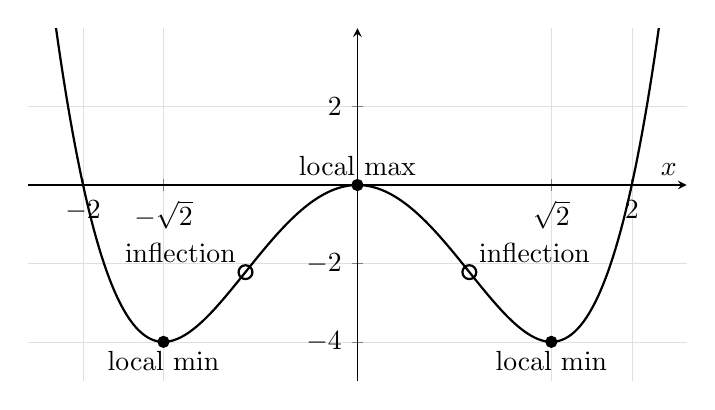
\begin{tikzpicture}
\begin{axis}[
    width=0.82\textwidth,
    height=0.50\textwidth,
    xmin=-2.4, xmax=2.4,
    ymin=-5, ymax=4,
    axis lines=middle,
    xlabel={\(x\)},
    ylabel={},
    xtick={-2,-1.414,0,1.414,2},
    xticklabels={\(-2\),\(-\sqrt2\),\(0\),\(\sqrt2\),\(2\)},
    ytick={-4,-2,0,2},
    grid=both,
    grid style={line width=.1pt, draw=gray!25},
]
\addplot[thick, domain=-2.2:2.2, samples=250] {x^4-4*x^2};

\addplot[only marks, mark=*] coordinates {(-1.414,-4) (0,0) (1.414,-4)};
\addplot[only marks, mark=o, mark size=2.5pt, thick] coordinates {(-0.816,-2.222) (0.816,-2.222)};

\node[anchor=north] at (axis cs:-1.414,-4) {local min};
\node[anchor=south] at (axis cs:0,0) {local max};
\node[anchor=north] at (axis cs:1.414,-4) {local min};

\node[anchor=south east] at (axis cs:-0.816,-2.222) {inflection};
\node[anchor=south west] at (axis cs:0.816,-2.222) {inflection};
\end{axis}
\end{tikzpicture}
\caption{The first derivative locates turning behavior.  The second derivative locates bending behavior.}
\label{fig:quartic-sign-chart-sketch}
\end{figure}

The exact function values at the turning points are

\[
f(-\sqrt2)=(-\sqrt2)^4-4(-\sqrt2)^2=4-8=-4,
\]

\[
f(0)=0,
\]

and

\[
f(\sqrt2)=(\sqrt2)^4-4(\sqrt2)^2=4-8=-4.
\]

The exact inflection points are

\[
\left(-\sqrt{\frac23},-\frac{20}{9}\right)
\qquad\text{and}\qquad
\left(\sqrt{\frac23},-\frac{20}{9}\right),
\]

because

\[
f\left(\pm\sqrt{\frac23}\right)
=
\left(\frac23\right)^2-4\left(\frac23\right)
=
\frac49-\frac83
=
-\frac{20}{9}.
\]

The picture is now almost forced.  The graph must fall to a low point, rise to a high
point, fall to another low point, and rise again.  It must bend upward, then downward,
then upward.

\[
\boxed{
\text{The sketch follows the sign charts.}
}
\]

\subsection{Asymptotes and end behavior}
\label{subsec:asymptotes-end-behavior}

Polynomials do not have vertical asymptotes.  Rational functions often do.

Derivative information describes shape where the function exists.  Limits describe what
happens near missing points and far away.

\begin{quote}
\textbf{Vertical asymptote.}
A line

\[
x=a
\]

is a \emph{vertical asymptote} of the graph of \(f\) if at least one of the one-sided
limits

\[
\lim_{x\to a^-} f(x),
\qquad
\lim_{x\to a^+} f(x)
\]

is \(+\infty\) or \(-\infty\).
\end{quote}

\paragraph{Example.}
For

\[
f(x)=\frac1{x-2},
\]

the denominator approaches \(0\) as \(x\to2\).  From the right,

\[
x-2>0,
\]

so

\[
f(x)\to+\infty.
\]

From the left,

\[
x-2<0,
\]

so

\[
f(x)\to-\infty.
\]

Therefore

\[
x=2
\]

is a vertical asymptote.

\begin{quote}
\textbf{Horizontal asymptote.}
A line

\[
y=L
\]

is a \emph{horizontal asymptote} as \(x\to\infty\) if

\[
\lim_{x\to\infty} f(x)=L.
\]

It is a horizontal asymptote as \(x\to-\infty\) if

\[
\lim_{x\to-\infty} f(x)=L.
\]
\end{quote}

\paragraph{Example.}
For

\[
g(x)=\frac{2x^2+1}{x^2+1},
\]

divide numerator and denominator by \(x^2\):

\[
g(x)=\frac{2+\frac1{x^2}}{1+\frac1{x^2}}.
\]

As \(x\to\pm\infty\),

\[
\frac1{x^2}\to0.
\]

So

\[
\lim_{x\to\pm\infty}g(x)=\frac{2+0}{1+0}=2.
\]

Therefore

\[
y=2
\]

is a horizontal asymptote.

Some graphs approach a slanted line instead of a horizontal line.

\begin{quote}
\textbf{Slant asymptote.}
A line

\[
y=mx+b
\]

is a \emph{slant asymptote} as \(x\to\infty\) if

\[
\lim_{x\to\infty}\bigl(f(x)-(mx+b)\bigr)=0.
\]

The same definition applies as \(x\to-\infty\).
\end{quote}

\paragraph{Example.}
Let

\[
h(x)=\frac{x^3}{x^2-1}.
\]

Divide:

\[
\frac{x^3}{x^2-1}
=
x+\frac{x}{x^2-1}.
\]

Since

\[
\frac{x}{x^2-1}\to0
\]

as \(x\to\pm\infty\), the graph approaches

\[
y=x.
\]

So \(y=x\) is a slant asymptote.

End behavior asks what happens as \(x\) becomes very large positive or very large
negative.  For this function, the end behavior is:

\[
h(x)\sim x
\quad\text{as}\quad
x\to\pm\infty.
\]

The symbol \(\sim\) here means that the two expressions have the same leading
behavior.  The difference between them approaches \(0\).

\subsection{A complete curve-sketching workflow}
\label{subsec:complete-curve-sketching-workflow}

A calculus sketch should gather evidence in an organized way.

\begin{quote}
\textbf{Curve-sketching workflow.}

\[
\begin{array}{ll}
\text{1.} & \text{Find the domain.}\\
\text{2.} & \text{Look for symmetry and intercepts.}\\
\text{3.} & \text{Find asymptotes and end behavior with limits.}\\
\text{4.} & \text{Compute } f'(x) \text{ and make a sign chart.}\\
\text{5.} & \text{Use } f' \text{ to find increasing/decreasing intervals and local extrema.}\\
\text{6.} & \text{Compute } f''(x) \text{ and make a sign chart.}\\
\text{7.} & \text{Use } f'' \text{ to find concavity and inflection points.}\\
\text{8.} & \text{Plot reliable points and sketch a graph that obeys all the evidence.}
\end{array}
\]
\end{quote}

The workflow is not a rigid machine.  Sometimes symmetry saves work.  Sometimes a
limit matters more than a derivative.  Sometimes a derivative is too complicated to
factor nicely.  But the questions are steady.

\paragraph{Example.}
Sketch

\[
f(x)=\frac{x^3}{x^2-1}.
\]

\paragraph{1. Domain.}
The denominator is zero when

\[
x^2-1=0,
\]

so

\[
x=\pm1.
\]

Thus the domain is

\[
(-\infty,-1)\cup(-1,1)\cup(1,\infty).
\]

The graph may break at \(x=-1\) and \(x=1\).

\paragraph{2. Symmetry and intercepts.}
Check symmetry:

\[
f(-x)=\frac{(-x)^3}{(-x)^2-1}
=
-\frac{x^3}{x^2-1}
=
-f(x).
\]

So \(f\) is odd.  The graph has origin symmetry.

The numerator is zero when

\[
x^3=0,
\]

so

\[
x=0.
\]

Therefore the graph has intercept

\[
(0,0).
\]

\paragraph{3. Asymptotes and end behavior.}
The possible vertical asymptotes are

\[
x=-1
\qquad\text{and}\qquad
x=1.
\]

Near \(x=1\), the numerator is positive and close to \(1\).  The denominator
\(x^2-1=(x-1)(x+1)\) changes sign.

Thus

\[
\lim_{x\to1^-}\frac{x^3}{x^2-1}=-\infty,
\]

and

\[
\lim_{x\to1^+}\frac{x^3}{x^2-1}=+\infty.
\]

Near \(x=-1\), the numerator is negative and close to \(-1\).  The denominator
again changes sign.  Therefore

\[
\lim_{x\to-1^-}\frac{x^3}{x^2-1}=-\infty,
\]

and

\[
\lim_{x\to-1^+}\frac{x^3}{x^2-1}=+\infty.
\]

So

\[
x=-1
\qquad\text{and}\qquad
x=1
\]

are vertical asymptotes.

For end behavior, divide:

\[
\frac{x^3}{x^2-1}
=
x+\frac{x}{x^2-1}.
\]

Since

\[
\frac{x}{x^2-1}\to0
\]

as \(x\to\pm\infty\), the graph has slant asymptote

\[
y=x.
\]

\paragraph{4. First derivative.}
Differentiate:

\[
f'(x)
=
\frac{(x^2-1)(3x^2)-x^3(2x)}{(x^2-1)^2}.
\]

Simplify:

\[
f'(x)
=
\frac{3x^4-3x^2-2x^4}{(x^2-1)^2}
=
\frac{x^4-3x^2}{(x^2-1)^2}.
\]

So

\[
f'(x)=\frac{x^2(x^2-3)}{(x^2-1)^2}.
\]

The denominator is positive wherever the function is defined.  The factor \(x^2\) is
nonnegative and is zero only at \(x=0\).  So the sign of \(f'\), away from \(x=0\),
comes from

\[
x^2-3.
\]

The critical numbers in the domain are

\[
x=-\sqrt3,\qquad x=0,\qquad x=\sqrt3.
\]

The domain breaks at

\[
x=-1,\qquad x=1.
\]

The sign chart is

\[
\begin{array}{c|cccccc}
\text{interval}
& (-\infty,-\sqrt3)
& (-\sqrt3,-1)
& (-1,0)
& (0,1)
& (1,\sqrt3)
& (\sqrt3,\infty) \\ \hline
f'(x)
& +
& -
& -
& -
& -
& + \\[2pt]
f
& \text{inc.}
& \text{dec.}
& \text{dec.}
& \text{dec.}
& \text{dec.}
& \text{inc.}
\end{array}
\]

Therefore \(f\) has a local maximum at

\[
x=-\sqrt3
\]

and a local minimum at

\[
x=\sqrt3.
\]

The values are

\[
f(-\sqrt3)
=
\frac{(-\sqrt3)^3}{(-\sqrt3)^2-1}
=
\frac{-3\sqrt3}{2},
\]

and

\[
f(\sqrt3)
=
\frac{(\sqrt3)^3}{(\sqrt3)^2-1}
=
\frac{3\sqrt3}{2}.
\]

At \(x=0\), we have

\[
f'(0)=0,
\]

but the sign of \(f'\) is negative on both sides of \(0\) inside the domain.  So there
is no local extremum at \(0\).

\paragraph{5. Second derivative.}
Differentiate again.  After simplification,

\[
f''(x)=\frac{2x(x^2+3)}{(x^2-1)^3}.
\]

Since

\[
x^2+3>0
\]

for every \(x\), the sign of \(f''\) comes from

\[
\frac{x}{(x^2-1)^3}.
\]

The concavity chart is

\[
\begin{array}{c|cccc}
\text{interval} & (-\infty,-1) & (-1,0) & (0,1) & (1,\infty) \\ \hline
f''(x) & - & + & - & + \\
f & \text{concave down} & \text{concave up} & \text{concave down} & \text{concave up}
\end{array}
\]

The concavity changes at \(x=0\), and \(f\) is continuous there.  Therefore

\[
(0,0)
\]

is an inflection point.  It is also a horizontal inflection point, because

\[
f'(0)=0.
\]

\paragraph{6. Sketch.}
The graph must obey all the evidence:

\[
\begin{array}{l}
\text{vertical asymptotes at }x=-1\text{ and }x=1,\\
\text{slant asymptote }y=x,\\
\text{origin symmetry,}\\
\text{local maximum at }\left(-\sqrt3,-\dfrac{3\sqrt3}{2}\right),\\[6pt]
\text{local minimum at }\left(\sqrt3,\dfrac{3\sqrt3}{2}\right),\\[6pt]
\text{horizontal inflection point at }(0,0).
\end{array}
\]

\begin{figure}[h]
\centering
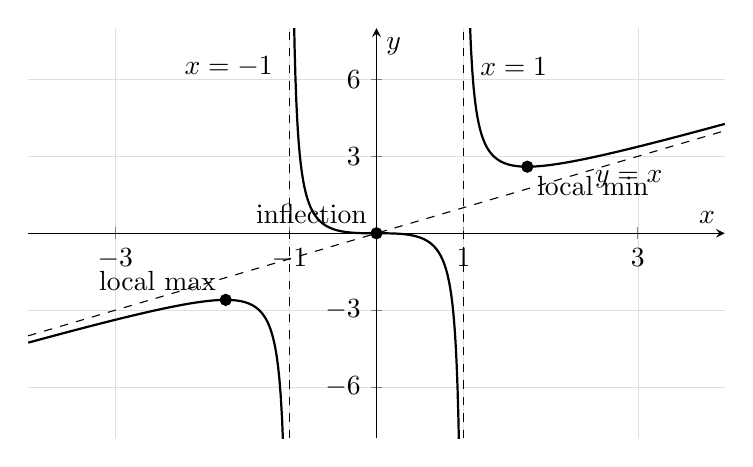
\begin{tikzpicture}
\begin{axis}[
    width=0.86\textwidth,
    height=0.56\textwidth,
    xmin=-4, xmax=4,
    ymin=-8, ymax=8,
    axis lines=middle,
    xlabel={\(x\)},
    ylabel={\(y\)},
    xtick={-3,-1,0,1,3},
    ytick={-6,-3,0,3,6},
    grid=both,
    grid style={line width=.1pt, draw=gray!25},
    clip=true,
]
% function branches
\addplot[thick, domain=-4:-1.04, samples=200] {x^3/(x^2-1)};
\addplot[thick, domain=-0.96:0.96, samples=200] {x^3/(x^2-1)};
\addplot[thick, domain=1.04:4, samples=200] {x^3/(x^2-1)};

% asymptotes
\addplot[dashed, domain=-4:4, samples=2] {x};
\draw[dashed] (axis cs:-1,-8) -- (axis cs:-1,8);
\draw[dashed] (axis cs:1,-8) -- (axis cs:1,8);

% important points
\addplot[only marks, mark=*] coordinates {(-1.732,-2.598) (0,0) (1.732,2.598)};
\node[anchor=south east] at (axis cs:-1.732,-2.598) {local max};
\node[anchor=north west] at (axis cs:1.732,2.598) {local min};
\node[anchor=south east] at (axis cs:0,0) {inflection};
\node[anchor=west] at (axis cs:2.4,2.1) {\(y=x\)};
\node[anchor=west] at (axis cs:1.08,6.5) {\(x=1\)};
\node[anchor=east] at (axis cs:-1.08,6.5) {\(x=-1\)};
\end{axis}
\end{tikzpicture}
\caption{A calculus sketch combines asymptotes, first derivative signs, and second derivative signs.}
\label{fig:rational-complete-sketch}
\end{figure}

The sketch is not only a picture of the formula.  It is a picture of the evidence.

\subsection{When technology helps and when it misleads}
\label{subsec:technology-helps-misleads-graphing}

A graphing calculator or computer can help check a sketch, but it should not replace
the analysis.

Technology draws what it samples.  It can miss a hole, hide an asymptote, or make a
bad viewing window look convincing.

\paragraph{A hidden hole.}
Consider

\[
p(x)=\frac{x^2-1}{x-1}.
\]

For \(x\neq1\),

\[
p(x)=x+1.
\]

A graphing device may draw the line

\[
y=x+1
\]

without showing the missing point at

\[
(1,2).
\]

But the original function is not defined at \(x=1\).  The correct graph is a line with a
hole.

\[
\boxed{
\text{Algebra and domain information can reveal what a plotted graph hides.}
}
\]

\paragraph{A misleading window.}
The function

\[
f(x)=\frac{x^3}{x^2-1}
\]

has vertical asymptotes at \(x=-1\) and \(x=1\).  But if we only graph it on the
window

\[
-0.8\le x\le0.8,
\]

we see only the middle branch.  The graph may look like a small decreasing curve
with a flat point at the origin.  That window hides the asymptotes and the outer
branches.

A graphing device answers the question we ask it.  Calculus helps us ask better
questions:

\[
\text{Where is the domain broken?}
\]

\[
\text{What happens near the broken points?}
\]

\[
\text{What happens as }x\to\pm\infty?
\]

\[
\text{What do }f'\text{ and }f''\text{ say?}
\]

A good sketch uses both tools: computation for speed, and calculus for judgment.

\subsection{Where this points}
\label{subsec:graph-sketching-hook-lhospital}

Graph sketching often leads back to limits.  A vertical asymptote is a limit.  A
horizontal or slant asymptote is a limit.  End behavior is a limit.

Some limits are easy.  Others have a strange form.  For example,

\[
\lim_{x\to1}\frac{\ln x}{x-1}
\]

has numerator and denominator both approaching \(0\).  The quotient could approach
a number, blow up, or fail to settle.

The next section gives a derivative-based tool for such limits.  Once again, local
linear approximation will explain the rule.

\section{Indeterminate forms and l'Hospital's Rule}
\label{sec:lhospitals-rule}

The last section used limits to find asymptotes and end behavior.  Some of those limits
can be read from algebra.  Others resist direct substitution.

Consider

\[
\lim_{x\to1}\frac{\ln x}{x-1}.
\]

Direct substitution gives

\[
\frac{\ln 1}{1-1}=\frac00.
\]

That expression is not a number.  It is a warning: both numerator and denominator
are approaching \(0\), and we need more information.

The derivative gives that information.

\subsection{The forms \(0/0\) and \(\infty/\infty\)}
\label{subsec:forms-zero-zero-infty-infty}

A quotient has the indeterminate form \(0/0\) if

\[
f(x)\to0
\qquad\text{and}\qquad
g(x)\to0.
\]

Then

\[
\frac{f(x)}{g(x)}
\]

may approach many different things.

For example, as \(x\to0\),

\[
\frac{x}{x}\to1,
\]

\[
\frac{x^2}{x}\to0,
\]

\[
\frac{x}{x^2}\to+\infty \quad \text{from the right},
\]

and

\[
\frac{5x}{x}\to5.
\]

All four quotients have the formal shape \(0/0\), but their limits behave differently.

\[
\boxed{
0/0 \text{ is not an answer.  It is a signal that more work is needed.}
}
\]

A quotient has the indeterminate form \(\infty/\infty\) if

\[
|f(x)|\to\infty
\qquad\text{and}\qquad
|g(x)|\to\infty.
\]

Again, the form alone does not decide the limit.

As \(x\to\infty\),

\[
\frac{x}{x}\to1,
\]

\[
\frac{x}{x^2}\to0,
\]

and

\[
\frac{x^2}{x}\to\infty.
\]

The numerator and denominator both grow without bound in all three examples, but
the ratios are different.

\subsection{Why derivatives can reveal a limiting ratio}
\label{subsec:derivatives-reveal-limiting-ratio}

Return to

\[
\lim_{x\to1}\frac{\ln x}{x-1}.
\]

Both numerator and denominator vanish at \(x=1\):

\[
\ln 1=0,
\qquad
1-1=0.
\]

But near \(x=1\), local linear approximation says

\[
\ln x
\approx
\ln 1+\left.\frac{d}{dx}\ln x\right|_{x=1}(x-1).
\]

Since

\[
\ln 1=0
\]

and

\[
\left.\frac{d}{dx}\ln x\right|_{x=1}=1,
\]

we get

\[
\ln x\approx x-1.
\]

So the quotient should satisfy

\[
\frac{\ln x}{x-1}\approx \frac{x-1}{x-1}=1.
\]

Thus

\[
\lim_{x\to1}\frac{\ln x}{x-1}=1.
\]

This is the idea behind l'Hospital's Rule.

When both functions vanish at the same point, their leading linear parts may decide
the limiting ratio:

\[
f(x)\approx f'(a)(x-a),
\]

\[
g(x)\approx g'(a)(x-a).
\]

Then

\[
\frac{f(x)}{g(x)}
\approx
\frac{f'(a)(x-a)}{g'(a)(x-a)}
=
\frac{f'(a)}{g'(a)}.
\]

This reasoning is not a proof in every case, because sometimes the first derivatives
also vanish or the point is approached from infinity.  But it gives the right reason for
the rule.

\subsection{l'Hospital's Rule}
\label{subsec:lhospital-statement}

\begin{quote}
\textbf{l'Hospital's Rule.}
Suppose \(f\) and \(g\) are differentiable near \(a\), except possibly at \(a\), and suppose

\[
g'(x)\neq0
\]

near \(a\).  If

\[
\lim_{x\to a}f(x)=0
\qquad\text{and}\qquad
\lim_{x\to a}g(x)=0,
\]

or if

\[
|f(x)|\to\infty
\qquad\text{and}\qquad
|g(x)|\to\infty,
\]

then, provided the limit on the right exists,

\[
\boxed{
\lim_{x\to a}\frac{f(x)}{g(x)}
=
\lim_{x\to a}\frac{f'(x)}{g'(x)}.
}
\]

The same rule applies to one-sided limits and to limits as \(x\to\infty\) or
\(x\to-\infty\), when the corresponding hypotheses hold.
\end{quote}

The rule says that, for the indeterminate forms \(0/0\) and \(\infty/\infty\), we may
replace the ratio of functions by the ratio of derivatives.

It does \emph{not} say that every quotient has the same limit as the quotient of its
derivatives.

\paragraph{Example.}
Find

\[
\lim_{x\to0}\frac{e^x-1}{x}.
\]

Direct substitution gives

\[
\frac{0}{0}.
\]

Differentiate numerator and denominator:

\[
\frac{d}{dx}(e^x-1)=e^x,
\qquad
\frac{d}{dx}(x)=1.
\]

Therefore

\[
\lim_{x\to0}\frac{e^x-1}{x}
=
\lim_{x\to0}\frac{e^x}{1}
=
1.
\]

This agrees with the local linear approximation

\[
e^x\approx1+x
\]

near \(x=0\).

\paragraph{Example.}
Find

\[
\lim_{x\to0}\frac{1-\cos x}{x^2}.
\]

Direct substitution gives \(0/0\).  Apply l'Hospital's Rule:

\[
\lim_{x\to0}\frac{1-\cos x}{x^2}
=
\lim_{x\to0}\frac{\sin x}{2x}.
\]

This is still \(0/0\).  Apply the rule again:

\[
\lim_{x\to0}\frac{\sin x}{2x}
=
\lim_{x\to0}\frac{\cos x}{2}
=
\frac12.
\]

So

\[
\boxed{
\lim_{x\to0}\frac{1-\cos x}{x^2}=\frac12.
}
\]

The first application did not finish the problem.  It made a new quotient.  Since the
new quotient was still indeterminate, a second application was allowed.

\paragraph{Example.}
Find

\[
\lim_{x\to\infty}\frac{x^2}{e^x}.
\]

Both numerator and denominator go to infinity, so this is the form \(\infty/\infty\).
Apply l'Hospital's Rule:

\[
\lim_{x\to\infty}\frac{x^2}{e^x}
=
\lim_{x\to\infty}\frac{2x}{e^x}.
\]

This is still \(\infty/\infty\).  Apply the rule again:

\[
\lim_{x\to\infty}\frac{2x}{e^x}
=
\lim_{x\to\infty}\frac{2}{e^x}
=
0.
\]

Thus

\[
\boxed{
\lim_{x\to\infty}\frac{x^2}{e^x}=0.
}
\]

The exponential eventually outruns the polynomial.

\subsection{Idea of the proof}
\label{subsec:lhospital-proof-idea}

The proof of l'Hospital's Rule comes from the Mean Value Theorem.  The cleanest
form uses a slightly stronger version called Cauchy's Mean Value Theorem.

\begin{quote}
\textbf{Cauchy's Mean Value Theorem.}
Suppose \(f\) and \(g\) are continuous on \([a,b]\) and differentiable on \((a,b)\).
Then there is some \(c\in(a,b)\) such that

\[
\bigl(f(b)-f(a)\bigr)g'(c)
=
\bigl(g(b)-g(a)\bigr)f'(c).
\]

If \(g'(c)\neq0\) and \(g(b)\neq g(a)\), this can be written as

\[
\frac{f(b)-f(a)}{g(b)-g(a)}
=
\frac{f'(c)}{g'(c)}.
\]
\end{quote}

\paragraph{Why Cauchy's theorem is true.}
Consider the function

\[
H(x)=\bigl(f(b)-f(a)\bigr)\bigl(g(x)-g(a)\bigr)
-
\bigl(g(b)-g(a)\bigr)\bigl(f(x)-f(a)\bigr).
\]

At \(x=a\),

\[
H(a)=0.
\]

At \(x=b\), the two products are equal, so

\[
H(b)=0.
\]

By Rolle's Theorem, there is some \(c\in(a,b)\) such that

\[
H'(c)=0.
\]

Differentiating \(H\) gives exactly

\[
\bigl(f(b)-f(a)\bigr)g'(c)
=
\bigl(g(b)-g(a)\bigr)f'(c).
\]

That is Cauchy's theorem.

\paragraph{How it proves the \(0/0\) case.}
Suppose

\[
f(a)=0,
\qquad
g(a)=0,
\]

and \(x\) is close to \(a\).  Apply Cauchy's Mean Value Theorem on the interval
from \(a\) to \(x\).  There is a point \(c\) between \(a\) and \(x\) such that

\[
\frac{f(x)-f(a)}{g(x)-g(a)}
=
\frac{f'(c)}{g'(c)}.
\]

Since

\[
f(a)=g(a)=0,
\]

this becomes

\[
\frac{f(x)}{g(x)}
=
\frac{f'(c)}{g'(c)}.
\]

As \(x\to a\), the point \(c\) is squeezed toward \(a\).  Therefore, if

\[
\frac{f'(c)}{g'(c)}\to L,
\]

then

\[
\frac{f(x)}{g(x)}\to L.
\]

So

\[
\lim_{x\to a}\frac{f(x)}{g(x)}
=
\lim_{x\to a}\frac{f'(x)}{g'(x)}.
\]

This proves the main idea for the \(0/0\) case.  The \(\infty/\infty\) case and endpoint
versions require more care, but the same Mean Value Theorem idea is behind them.

\subsection{Other indeterminate forms}
\label{subsec:other-indeterminate-forms}

The forms \(0/0\) and \(\infty/\infty\) are the ones l'Hospital's Rule handles directly.
Other indeterminate forms can often be rewritten into one of those two forms.

Common forms include

\[
0\cdot\infty,
\qquad
\infty-\infty,
\qquad
0^0,
\qquad
1^\infty,
\qquad
\infty^0.
\]

Each one needs algebra before l'Hospital's Rule can be used.

\paragraph{A \(0\cdot\infty\) form.}
Find

\[
\lim_{x\to0^+}x\ln x.
\]

As \(x\to0^+\),

\[
x\to0
\]

and

\[
\ln x\to-\infty.
\]

So this has the form \(0\cdot(-\infty)\).  Rewrite it as a quotient:

\[
x\ln x=\frac{\ln x}{1/x}.
\]

Now the numerator and denominator both grow in magnitude:

\[
\ln x\to-\infty,
\qquad
\frac1x\to+\infty.
\]

Apply l'Hospital's Rule:

\[
\lim_{x\to0^+}\frac{\ln x}{1/x}
=
\lim_{x\to0^+}
\frac{1/x}{-1/x^2}
=
\lim_{x\to0^+}(-x)
=
0.
\]

Therefore

\[
\boxed{
\lim_{x\to0^+}x\ln x=0.
}
\]

The product approaches \(0\), even though one factor approaches \(-\infty\).

\paragraph{An \(\infty-\infty\) form.}
Find

\[
\lim_{x\to0}\left(\frac1x-\frac1{e^x-1}\right).
\]

Each term blows up as \(x\to0\), so this is an \(\infty-\infty\) form.  Put the terms
over a common denominator:

\[
\frac1x-\frac1{e^x-1}
=
\frac{e^x-1-x}{x(e^x-1)}.
\]

Now direct substitution gives \(0/0\).  Apply l'Hospital's Rule:

\[
\lim_{x\to0}
\frac{e^x-1-x}{x(e^x-1)}
=
\lim_{x\to0}
\frac{e^x-1}{(e^x-1)+xe^x}.
\]

This is still \(0/0\).  Apply the rule again:

\[
\lim_{x\to0}
\frac{e^x}{e^x+e^x+xe^x}
=
\lim_{x\to0}
\frac{e^x}{(2+x)e^x}
=
\frac12.
\]

Thus

\[
\boxed{
\lim_{x\to0}\left(\frac1x-\frac1{e^x-1}\right)=\frac12.
}
\]

The subtraction hides a cancellation.  Algebra exposes it.

\paragraph{A power form \(0^0\).}
Find

\[
\lim_{x\to0^+}x^x.
\]

The base approaches \(0\), and the exponent approaches \(0\), so this has the form
\(0^0\).  Power forms are usually handled by taking logarithms.

Let

\[
y=x^x.
\]

Then

\[
\ln y=x\ln x.
\]

We just found that

\[
\lim_{x\to0^+}x\ln x=0.
\]

Therefore

\[
\lim_{x\to0^+}\ln y=0.
\]

Since the exponential function is continuous,

\[
\lim_{x\to0^+}y=e^0=1.
\]

So

\[
\boxed{
\lim_{x\to0^+}x^x=1.
}
\]

The expression \(0^0\) by itself did not decide the answer.  The limiting process did.

\paragraph{A power form \(1^\infty\).}
Find

\[
\lim_{x\to\infty}\left(1+\frac1x\right)^x.
\]

Let

\[
y=\left(1+\frac1x\right)^x.
\]

Then

\[
\ln y=x\ln\left(1+\frac1x\right).
\]

Set

\[
u=\frac1x.
\]

As \(x\to\infty\), we have \(u\to0^+\).  Also,

\[
x=\frac1u.
\]

Thus

\[
\ln y
=
\frac{\ln(1+u)}{u}.
\]

This is \(0/0\).  Apply l'Hospital's Rule with respect to \(u\):

\[
\lim_{u\to0^+}\frac{\ln(1+u)}{u}
=
\lim_{u\to0^+}\frac{1/(1+u)}{1}
=
1.
\]

So

\[
\lim_{x\to\infty}\ln y=1.
\]

Therefore

\[
\lim_{x\to\infty}y=e.
\]

Thus

\[
\boxed{
\lim_{x\to\infty}\left(1+\frac1x\right)^x=e.
}
\]

This familiar limit now appears as a logarithmic indeterminate form.

\subsection{Comparing growth rates}
\label{subsec:comparing-growth-rates}

l'Hospital's Rule gives a clean way to compare common growth rates.

\paragraph{Logarithms grow slower than powers.}
Let \(p>0\).  Then

\[
\lim_{x\to\infty}\frac{\ln x}{x^p}
\]

has form \(\infty/\infty\).  Apply l'Hospital's Rule:

\[
\lim_{x\to\infty}\frac{\ln x}{x^p}
=
\lim_{x\to\infty}\frac{1/x}{p x^{p-1}}
=
\lim_{x\to\infty}\frac1{p x^p}
=
0.
\]

So

\[
\boxed{
\ln x \text{ grows slower than } x^p \text{ for every } p>0.
}
\]

\paragraph{Powers grow slower than exponentials.}
Let \(n\) be a positive integer.  Consider

\[
\lim_{x\to\infty}\frac{x^n}{e^x}.
\]

Apply l'Hospital's Rule \(n\) times:

\[
\frac{x^n}{e^x}
\longrightarrow
\frac{n x^{n-1}}{e^x}
\longrightarrow
\frac{n(n-1)x^{n-2}}{e^x}
\longrightarrow
\cdots
\longrightarrow
\frac{n!}{e^x}.
\]

Since

\[
\frac{n!}{e^x}\to0,
\]

we get

\[
\boxed{
\lim_{x\to\infty}\frac{x^n}{e^x}=0.
}
\]

So exponentials eventually grow faster than powers.

A rough hierarchy is

\[
\ln x
\quad\ll\quad
x^p
\quad\ll\quad
e^x
\]

as \(x\to\infty\), for \(p>0\).  The symbol \(\ll\) means ``grows much more slowly
than'' in this limiting sense.

This hierarchy will return when we study infinite series and Taylor approximation.
Growth rate decides convergence, error size, and which terms dominate.

\subsection{When l'Hospital's Rule cannot be used}
\label{subsec:lhospital-cannot-be-used}

l'Hospital's Rule is easy to misuse.  The first check is always the form.

\paragraph{Not an indeterminate form.}
Consider

\[
\lim_{x\to0}\frac{x^2+1}{x+1}.
\]

Direct substitution gives

\[
\frac{1}{1}=1.
\]

This is not \(0/0\) or \(\infty/\infty\).  The limit is \(1\).

If we incorrectly differentiate numerator and denominator, we get

\[
\lim_{x\to0}\frac{2x}{1}=0,
\]

which is the wrong answer.

\[
\boxed{
\text{Do not use l'Hospital's Rule unless the quotient has form }0/0
\text{ or }\infty/\infty.
}
\]

\paragraph{Derivative quotient has no limit.}
Sometimes l'Hospital's Rule gives no conclusion, even though the original limit exists.

Consider

\[
\lim_{x\to\infty}\frac{x+\sin x}{x}.
\]

The original quotient is

\[
\frac{x+\sin x}{x}
=
1+\frac{\sin x}{x}.
\]

Since

\[
\left|\frac{\sin x}{x}\right|\le \frac1x,
\]

we have

\[
\frac{\sin x}{x}\to0.
\]

Thus

\[
\lim_{x\to\infty}\frac{x+\sin x}{x}=1.
\]

But the quotient of derivatives is

\[
\frac{1+\cos x}{1}=1+\cos x,
\]

which has no limit as \(x\to\infty\).

There is no contradiction.  l'Hospital's Rule says that if the derivative quotient has a
limit, then the original quotient has that same limit.  It does not say that the derivative
quotient must have a limit whenever the original quotient does.

\subsection{Where this points}
\label{subsec:lhospital-hook-warning-review}

l'Hospital's Rule turns some hard limits into derivative limits.  It works because, near
a point, differentiable functions are controlled by their local linear parts.

But every theorem in this chapter has boundaries.  Fermat's theorem needs an interior
point and differentiability.  The Mean Value Theorem needs continuity and
differentiability.  The second derivative test can be silent.  l'Hospital's Rule needs an
indeterminate form and a derivative quotient that settles.

The next warning examples collect those boundaries, because knowing when a theorem
cannot be used is part of knowing the theorem.
\section{Warning examples}
\label{sec:warning-examples-chapter-6}

The last few sections gave us strong tools:

\[
\text{Fermat's theorem, Rolle's theorem, the Mean Value Theorem,}
\]

\[
\text{the first derivative test, the second derivative test, and l'Hospital's Rule.}
\]

Each one has a boundary.  A theorem is useful only when its hypotheses are true.
This section collects the warning examples in one place, so the rules are easier to use
and harder to misuse.

\subsection{Fermat's theorem fails at an endpoint}
\label{subsec:fermat-endpoint-warning}

Fermat's theorem said:

\[
\text{differentiable local extremum at an interior point}
\quad\Longrightarrow\quad
f'(c)=0.
\]

The phrase \emph{interior point} matters.

Let

\[
f(x)=x
\]

on the interval

\[
[0,1].
\]

The function has an absolute minimum at

\[
x=0
\]

and an absolute maximum at

\[
x=1.
\]

But the derivative is

\[
f'(x)=1.
\]

There is no horizontal tangent.

\begin{figure}[h]
\centering
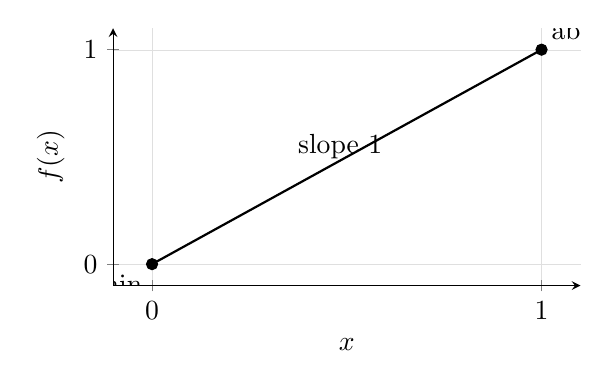
\begin{tikzpicture}
\begin{axis}[
    width=0.62\textwidth,
    height=0.40\textwidth,
    xmin=-0.1, xmax=1.1,
    ymin=-0.1, ymax=1.1,
    axis lines=left,
    xlabel={\(x\)},
    ylabel={\(f(x)\)},
    xtick={0,1},
    ytick={0,1},
    grid=both,
    grid style={line width=.1pt, draw=gray!25},
]
\addplot[thick, domain=0:1, samples=2] {x};
\addplot[only marks, mark=*] coordinates {(0,0) (1,1)};
\node[anchor=north east] at (axis cs:0,0) {absolute min};
\node[anchor=south west] at (axis cs:1,1) {absolute max};
\node[anchor=west] at (axis cs:0.35,0.55) {slope \(1\)};
\end{axis}
\end{tikzpicture}
\caption{An endpoint can be highest or lowest simply because the interval stops.}
\label{fig:fermat-endpoint-warning}
\end{figure}

There is no contradiction.  Fermat's theorem applies to interior points.  At an endpoint,
the graph only has to be compared with points on one side.  It can be best or worst
without flattening out.

\[
\boxed{
\text{Endpoint extrema do not have to satisfy } f'(c)=0.
}
\]

That is why the closed interval method always checks endpoints separately.

\subsection{The Mean Value Theorem fails without continuity}
\label{subsec:mvt-continuity-warning}

The Mean Value Theorem said that if \(f\) is continuous on \([a,b]\) and differentiable
on \((a,b)\), then some \(c\in(a,b)\) satisfies

\[
f'(c)=\frac{f(b)-f(a)}{b-a}.
\]

Continuity on the whole closed interval matters.

Define

\[
f(x)=
\begin{cases}
x, & 0\le x<1,\\
0, & x=1.
\end{cases}
\]

on \([0,1]\).

Then

\[
f(0)=0,
\qquad
f(1)=0.
\]

So the secant slope from \(0\) to \(1\) is

\[
\frac{f(1)-f(0)}{1-0}=0.
\]

But on the open interval \((0,1)\),

\[
f(x)=x,
\]

so

\[
f'(x)=1
\]

for every \(x\in(0,1)\).  There is no point \(c\in(0,1)\) with

\[
f'(c)=0.
\]

\begin{figure}[h]
\centering
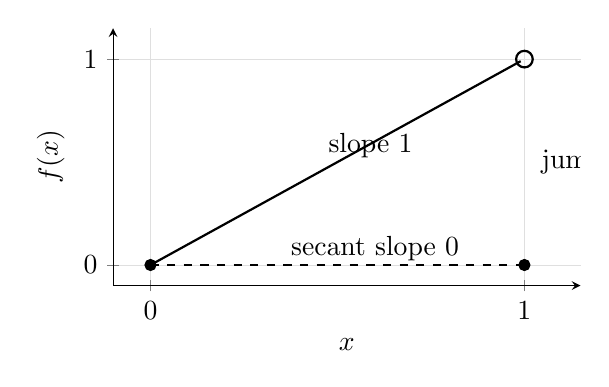
\begin{tikzpicture}
\begin{axis}[
    width=0.62\textwidth,
    height=0.40\textwidth,
    xmin=-0.1, xmax=1.15,
    ymin=-0.1, ymax=1.15,
    axis lines=left,
    xlabel={\(x\)},
    ylabel={\(f(x)\)},
    xtick={0,1},
    ytick={0,1},
    grid=both,
    grid style={line width=.1pt, draw=gray!25},
]
\addplot[thick, domain=0:0.99, samples=2] {x};
\addplot[only marks, mark=o, mark size=3pt, thick] coordinates {(1,1)};
\addplot[only marks, mark=*] coordinates {(0,0) (1,0)};
\addplot[dashed, domain=0:1, samples=2] {0};
\node[anchor=west] at (axis cs:0.45,0.58) {slope \(1\)};
\node[anchor=west] at (axis cs:0.35,0.08) {secant slope \(0\)};
\node[anchor=west] at (axis cs:1.02,0.5) {jump};
\end{axis}
\end{tikzpicture}
\caption{Without continuity, the endpoint secant slope may not appear as any tangent slope.}
\label{fig:mvt-continuity-warning}
\end{figure}

The graph climbs toward \(1\), then jumps down at the endpoint.  The jump hides the
climb from the endpoint calculation.

\[
\boxed{
\text{The Mean Value Theorem needs continuity on }[a,b].
}
\]

\subsection{The Mean Value Theorem fails without differentiability}
\label{subsec:mvt-differentiability-warning}

The Mean Value Theorem also needs differentiability on the open interval.

Let

\[
f(x)=|x|
\]

on

\[
[-1,1].
\]

The function is continuous on \([-1,1]\).  Its endpoint values are

\[
f(-1)=1,
\qquad
f(1)=1.
\]

So the secant slope is

\[
\frac{f(1)-f(-1)}{1-(-1)}
=
\frac{1-1}{2}
=
0.
\]

If the Mean Value Theorem applied, there would be some \(c\in(-1,1)\) with

\[
f'(c)=0.
\]

But

\[
f'(x)=-1
\quad\text{for }x<0,
\]

and

\[
f'(x)=1
\quad\text{for }x>0.
\]

At \(x=0\), the derivative does not exist.  The graph turns at a corner.

\begin{figure}[h]
\centering
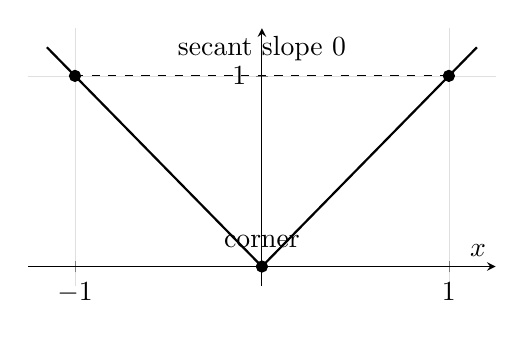
\begin{tikzpicture}
\begin{axis}[
    width=0.62\textwidth,
    height=0.40\textwidth,
    xmin=-1.25, xmax=1.25,
    ymin=-0.1, ymax=1.25,
    axis lines=middle,
    xlabel={\(x\)},
    ylabel={},
    xtick={-1,0,1},
    ytick={0,1},
    grid=both,
    grid style={line width=.1pt, draw=gray!25},
]
\addplot[thick, domain=-1.15:0, samples=2] {-x};
\addplot[thick, domain=0:1.15, samples=2] {x};
\addplot[dashed, domain=-1:1, samples=2] {1};
\addplot[only marks, mark=*] coordinates {(-1,1) (0,0) (1,1)};
\node[anchor=south] at (axis cs:0,0.05) {corner};
\node[anchor=south] at (axis cs:0,1.03) {secant slope \(0\)};
\end{axis}
\end{tikzpicture}
\caption{A corner can create a turn without any horizontal tangent.}
\label{fig:mvt-differentiability-warning}
\end{figure}

The graph does return to the same height, but it turns too sharply.  Rolle's Theorem
and the Mean Value Theorem do not promise a horizontal tangent unless the function
is differentiable throughout the open interval.

\[
\boxed{
\text{The Mean Value Theorem needs differentiability on }(a,b).
}
\]

\subsection{The second derivative test can be inconclusive}
\label{subsec:second-derivative-inconclusive-warning}

The second derivative test said:

\[
f'(c)=0,\quad f''(c)>0
\quad\Longrightarrow\quad
\text{local minimum at }c,
\]

and

\[
f'(c)=0,\quad f''(c)<0
\quad\Longrightarrow\quad
\text{local maximum at }c.
\]

But when

\[
f''(c)=0,
\]

the test says nothing.

Three different outcomes are possible.

\paragraph{A local minimum.}
Let

\[
f(x)=x^4.
\]

Then

\[
f'(x)=4x^3,
\qquad
f''(x)=12x^2.
\]

At \(x=0\),

\[
f'(0)=0,
\qquad
f''(0)=0.
\]

The second derivative test gives no conclusion.  But

\[
x^4\ge0
\]

for every \(x\), so \(f\) has a local minimum at \(0\).

\paragraph{A local maximum.}
Let

\[
g(x)=-x^4.
\]

Then

\[
g'(x)=-4x^3,
\qquad
g''(x)=-12x^2.
\]

At \(x=0\),

\[
g'(0)=0,
\qquad
g''(0)=0.
\]

The test again gives no conclusion.  But

\[
-x^4\le0
\]

for every \(x\), so \(g\) has a local maximum at \(0\).

\paragraph{No local extremum.}
Let

\[
h(x)=x^3.
\]

Then

\[
h'(x)=3x^2,
\qquad
h''(x)=6x.
\]

At \(x=0\),

\[
h'(0)=0,
\qquad
h''(0)=0.
\]

But \(x^3\) is increasing through \(0\).  There is no local maximum or local minimum.

\begin{figure}[h]
\centering
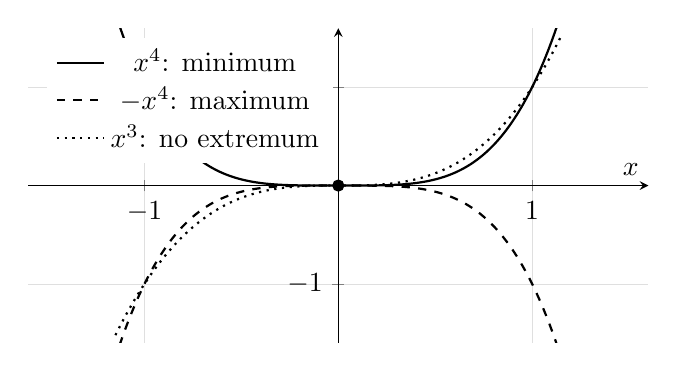
\begin{tikzpicture}
\begin{axis}[
    width=0.78\textwidth,
    height=0.46\textwidth,
    xmin=-1.6, xmax=1.6,
    ymin=-1.6, ymax=1.6,
    axis lines=middle,
    xlabel={\(x\)},
    ylabel={},
    xtick={-1,0,1},
    ytick={-1,0,1},
    grid=both,
    grid style={line width=.1pt, draw=gray!25},
    legend style={draw=none, at={(0.03,0.97)}, anchor=north west}
]
\addplot[thick, domain=-1.45:1.45, samples=200] {x^4};
\addlegendentry{\(x^4\): minimum}
\addplot[thick, dashed, domain=-1.45:1.45, samples=200] {-x^4};
\addlegendentry{\(-x^4\): maximum}
\addplot[thick, dotted, domain=-1.15:1.15, samples=200] {x^3};
\addlegendentry{\(x^3\): no extremum}
\addplot[only marks, mark=*] coordinates {(0,0)};
\end{axis}
\end{tikzpicture}
\caption{When \(f'(0)=0\) and \(f''(0)=0\), the second derivative test is silent.}
\label{fig:second-derivative-test-silent}
\end{figure}

The moral is short:

\[
\boxed{
f''(c)=0 \text{ means ``try another test.''}
}
\]

Most often, we return to the first derivative test or to the definition of local maximum
and local minimum.

\subsection{l'Hospital's Rule cannot be used on every quotient}
\label{subsec:lhospital-every-quotient-warning}

l'Hospital's Rule is a rule for the indeterminate forms

\[
\frac00
\qquad\text{and}\qquad
\frac{\infty}{\infty}.
\]

The first question is always:

\[
\text{What form does direct substitution produce?}
\]

\paragraph{A quotient that is not indeterminate.}
Consider

\[
\lim_{x\to0}\frac{x^2+1}{x+1}.
\]

Direct substitution gives

\[
\frac{0^2+1}{0+1}=1.
\]

So the limit is

\[
1.
\]

This is not a \(0/0\) form and not an \(\infty/\infty\) form.

If we incorrectly differentiate numerator and denominator, we get

\[
\lim_{x\to0}\frac{2x}{1}=0,
\]

which is wrong.

\[
\boxed{
\text{Do not use l'Hospital's Rule when direct substitution already gives an ordinary number.}
}
\]

\paragraph{A derivative quotient with no limit.}
Sometimes the original quotient has a limit, but the quotient of derivatives does not.

Consider

\[
\lim_{x\to\infty}\frac{x+\sin x}{x}.
\]

The quotient is

\[
\frac{x+\sin x}{x}
=
1+\frac{\sin x}{x}.
\]

Since

\[
\left|\frac{\sin x}{x}\right|\le \frac1x
\]

for \(x>0\), we get

\[
\frac{\sin x}{x}\to0.
\]

Therefore

\[
\lim_{x\to\infty}\frac{x+\sin x}{x}=1.
\]

But the quotient of derivatives is

\[
\frac{1+\cos x}{1}=1+\cos x,
\]

which has no limit as \(x\to\infty\).

There is no contradiction.  l'Hospital's Rule says that if the original quotient has the
right indeterminate form and the derivative quotient has a limit, then the original limit
has that same value.  It does not say that the derivative quotient must always have a
limit.

\[
\boxed{
\text{If the derivative quotient does not settle, l'Hospital's Rule gives no conclusion.}
}
\]

\subsection{A theorem-use checklist}
\label{subsec:chapter-6-theorem-checklist}

The warnings can be compressed into a practical checklist.

\[
\begin{array}{c|p{0.58\textwidth}}
\textbf{tool} & \textbf{check before using it} \\ \hline
\text{Fermat's theorem}
& Is the extremum at an interior point?  Is the function differentiable there? \\[4pt]

\text{Mean Value Theorem}
& Is the function continuous on \([a,b]\)?  Is it differentiable on \((a,b)\)? \\[4pt]

\text{first derivative test}
& Does \(f'\) actually change sign around the critical number? \\[4pt]

\text{second derivative test}
& Is \(f'(c)=0\)?  Is \(f''(c)\) positive or negative, not zero? \\[4pt]

\text{l'Hospital's Rule}
& Is the quotient really \(0/0\) or \(\infty/\infty\)?  Does the derivative quotient have a limit?
\end{array}
\]

A theorem is not only a conclusion.  It is a package:

\[
\text{hypotheses}
\quad\Longrightarrow\quad
\text{conclusion}.
\]

If the hypotheses are missing, the conclusion may still be true by luck.  But the theorem
is no longer the reason.

These warnings prepare the chapter review.  We now gather the ideas into one working
map: how to read shape from derivatives, how to prove global facts from the Mean Value
Theorem, and how to tell when a tempting shortcut is legal.

\section{Chapter review and discovery problems}
\label{sec:chapter-6-review-discovery}

This chapter began with a simple observation:

\[
f'(x)>0 \text{ means rising},
\qquad
f'(x)<0 \text{ means falling}.
\]

That observation grew into a much larger picture.  The derivative gives more than
instantaneous rate.  It gives shape, turning, bending, bounds, and sometimes limits.

\subsection{The chapter's map}
\label{subsec:chapter-6-map}

Here is the main dictionary.

\[
\begin{array}{c|c}
\textbf{calculus evidence} & \textbf{graph information} \\ \hline
f'(x)>0 & f \text{ is increasing} \\[3pt]
f'(x)<0 & f \text{ is decreasing} \\[3pt]
f'(c)=0 \text{ or } f'(c)\text{ undefined} & c \text{ is a critical number candidate} \\[3pt]
f' \text{ changes } + \text{ to } - & \text{local maximum} \\[3pt]
f' \text{ changes } - \text{ to } + & \text{local minimum} \\[3pt]
f''(x)>0 & f \text{ is concave up} \\[3pt]
f''(x)<0 & f \text{ is concave down} \\[3pt]
f'' \text{ changes sign at } c & (c,f(c)) \text{ is an inflection point} \\[3pt]
f'(c)=0,\ f''(c)>0 & \text{local minimum} \\[3pt]
f'(c)=0,\ f''(c)<0 & \text{local maximum}
\end{array}
\]

The Mean Value Theorem supplies the bridge from local derivative information to
whole-interval information:

\[
\boxed{
f'(c)=\frac{f(b)-f(a)}{b-a}
}
\]

for some

\[
c\in(a,b),
\]

provided \(f\) is continuous on \([a,b]\) and differentiable on \((a,b)\).

That bridge proves the first derivative sign rule.  It also proves that a function with
zero derivative on an interval is constant there.

l'Hospital's Rule is another derivative bridge.  For certain indeterminate quotients,
the limiting ratio of two functions can be found from the limiting ratio of their
derivatives:

\[
\lim_{x\to a}\frac{f(x)}{g(x)}
=
\lim_{x\to a}\frac{f'(x)}{g'(x)},
\]

when the hypotheses of the rule are satisfied.

\subsection{A complete review example}
\label{subsec:chapter-6-complete-review-example}

Sketch the graph of

\[
f(x)=\frac13x^3-x^2
\]

using derivatives.

First compute

\[
f'(x)=x^2-2x=x(x-2).
\]

The critical numbers are

\[
x=0
\qquad\text{and}\qquad
x=2.
\]

The sign chart for \(f'\) is

\[
\begin{array}{c|ccc}
\text{interval} & (-\infty,0) & (0,2) & (2,\infty) \\ \hline
f'(x) & + & - & + \\[2pt]
f & \text{increasing} & \text{decreasing} & \text{increasing}
\end{array}
\]

So \(f\) has a local maximum at \(x=0\) and a local minimum at \(x=2\).

The values are

\[
f(0)=0,
\]

and

\[
f(2)=\frac13(8)-4=\frac83-\frac{12}{3}=-\frac43.
\]

Now compute the second derivative:

\[
f''(x)=2x-2.
\]

The sign chart for \(f''\) is

\[
\begin{array}{c|cc}
\text{interval} & (-\infty,1) & (1,\infty) \\ \hline
f''(x) & - & + \\[2pt]
f & \text{concave down} & \text{concave up}
\end{array}
\]

The concavity changes at \(x=1\).  Therefore there is an inflection point at

\[
\left(1,f(1)\right)
=
\left(1,\frac13-1\right)
=
\left(1,-\frac23\right).
\]

The graph must rise to \((0,0)\), fall to \(\left(2,-\frac43\right)\), then rise again.
It bends downward before \(x=1\) and upward after \(x=1\).

\begin{figure}[h]
\centering
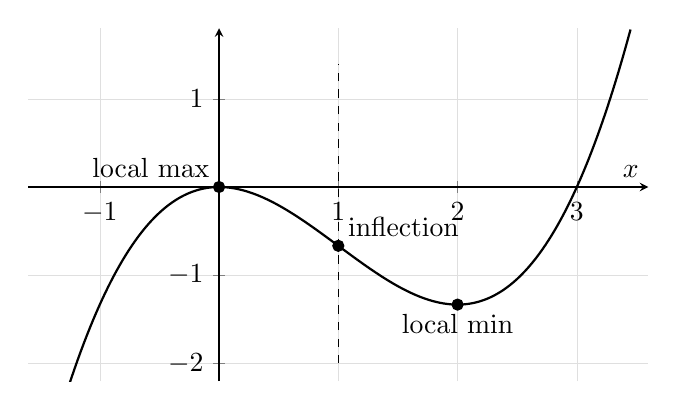
\begin{tikzpicture}
\begin{axis}[
    width=0.78\textwidth,
    height=0.50\textwidth,
    xmin=-1.6, xmax=3.6,
    ymin=-2.2, ymax=1.8,
    axis lines=middle,
    xlabel={\(x\)},
    ylabel={},
    xtick={-1,0,1,2,3},
    ytick={-2,-1,0,1},
    grid=both,
    grid style={line width=.1pt, draw=gray!25},
]
\addplot[thick, domain=-1.45:3.45, samples=200] {(x^3)/3-x^2};
\addplot[only marks, mark=*] coordinates {(0,0) (1,-0.6667) (2,-1.3333)};
\node[anchor=south east] at (axis cs:0,0) {local max};
\node[anchor=south west] at (axis cs:1,-0.6667) {inflection};
\node[anchor=north] at (axis cs:2,-1.3333) {local min};
\draw[dashed] (axis cs:1,-2.0) -- (axis cs:1,1.4);
\end{axis}
\end{tikzpicture}
\caption{A first derivative sign chart gives turning behavior.  A second derivative sign chart gives bending behavior.}
\label{fig:chapter-6-review-example}
\end{figure}

This example is small, but the workflow is the same for harder functions:

\[
\text{domain, intercepts, asymptotes, } f', f'', \text{ sign charts, then sketch.}
\]

\subsection{Concept checks}
\label{subsec:chapter-6-concept-checks}

\begin{enumerate}
\item Explain why a critical number is a candidate for a local extremum, not a
guarantee.

\item Give an example of a function with \(f'(0)=0\) but no local maximum or local
minimum at \(0\).

\item Give an example of a function with a local minimum at \(0\) where \(f'(0)\) does
not exist.

\item Explain why endpoints must be checked when finding absolute extrema on a
closed interval.

\item State the hypotheses of the Mean Value Theorem.  For each hypothesis, give one
sentence explaining why it is needed.

\item Suppose \(f'(x)>0\) for all \(x\) in an interval.  Explain why \(f\) cannot take the
same value twice in that interval.

\item Suppose \(f''(x)>0\) on an interval.  What does that say about \(f'\)?  What does
it say about the graph of \(f\)?

\item If \(f''(c)=0\), what can you conclude about local extrema at \(c\)?  What can you
not conclude?

\item Before applying l'Hospital's Rule, what two checks should be made?

\item Explain why

\[
\frac00
\]

is not a value of a limit.
\end{enumerate}

\subsection{Skills: graph from derivatives}
\label{subsec:skills-graph-from-derivatives}

For each function below:

\[
\begin{array}{ll}
\text{1.} & \text{Find the domain.}\\
\text{2.} & \text{Find intercepts, if reasonable.}\\
\text{3.} & \text{Find vertical, horizontal, or slant asymptotes, if any.}\\
\text{4.} & \text{Find critical numbers.}\\
\text{5.} & \text{Find increasing and decreasing intervals.}\\
\text{6.} & \text{Find local extrema.}\\
\text{7.} & \text{Find concavity intervals and inflection points.}\\
\text{8.} & \text{Sketch a graph consistent with all the evidence.}
\end{array}
\]

\begin{enumerate}
\item

\[
f(x)=x^3-6x^2+9x+1.
\]

\item

\[
f(x)=x^4-4x^2.
\]

\item

\[
f(x)=\frac{x}{x^2+1}.
\]

\item

\[
f(x)=\frac{x^2}{x-1}.
\]

\item

\[
f(x)=xe^{-x}.
\]

\item

\[
f(x)=\ln(x^2+1).
\]

\item

\[
f(x)=x+\frac1x,
\qquad x\neq0.
\]

\item

\[
f(x)=\frac{x^3}{x^2-1}.
\]

\item The derivative of a function \(f\) has sign chart

\[
\begin{array}{c|cccc}
\text{interval} & (-\infty,-2) & (-2,0) & (0,3) & (3,\infty) \\ \hline
f'(x) & - & + & + & -
\end{array}
\]

and \(f\) is continuous everywhere.  Identify all local extrema forced by the chart.

\item The second derivative of a function \(g\) has sign chart

\[
\begin{array}{c|ccc}
\text{interval} & (-\infty,1) & (1,4) & (4,\infty) \\ \hline
g''(x) & + & - & +
\end{array}
\]

and \(g\) is continuous everywhere.  Identify all inflection points forced by the chart.
\end{enumerate}

\subsection{Extrema and closed interval practice}
\label{subsec:chapter-6-extrema-practice}

\begin{enumerate}
\item Find the absolute maximum and minimum values of

\[
f(x)=x^3-3x+2
\]

on

\[
[-2,3].
\]

\item Find the absolute maximum and minimum values of

\[
g(x)=x+\frac4x
\]

on

\[
[1,6].
\]

\item Find the absolute maximum and minimum values of

\[
h(x)=\sqrt{x}(4-x)
\]

on

\[
[0,4].
\]

\item Let

\[
p(x)=x^4-8x^2+3.
\]

Find all local extrema and all absolute extrema on

\[
[-3,3].
\]

\item Explain why the function

\[
f(x)=\frac1x
\]

has no absolute maximum or minimum on

\[
(0,1).
\]

Which hypothesis of the Extreme Value Theorem is missing?

\item Explain why the function

\[
f(x)=x
\]

has no absolute maximum on

\[
[0,\infty).
\]

Which hypothesis of the Extreme Value Theorem is missing?
\end{enumerate}

\subsection{Mean Value Theorem practice}
\label{subsec:chapter-6-mvt-practice}

\begin{enumerate}
\item Verify the hypotheses of the Mean Value Theorem for

\[
f(x)=x^2
\]

on

\[
[1,4].
\]

Find all numbers \(c\in(1,4)\) satisfying

\[
f'(c)=\frac{f(4)-f(1)}{4-1}.
\]

\item Verify the hypotheses of Rolle's Theorem for

\[
f(x)=x^2-4x+3
\]

on

\[
[1,3].
\]

Find the number \(c\) promised by the theorem.

\item Let

\[
f(x)=\sqrt{x}
\]

on

\[
[1,9].
\]

Find the number \(c\) promised by the Mean Value Theorem.

\item Show that the Mean Value Theorem cannot be applied to

\[
f(x)=|x|
\]

on

\[
[-1,1].
\]

Then explain why the conclusion fails.

\item Show that the Mean Value Theorem cannot be applied to

\[
f(x)=
\begin{cases}
x, & 0\le x<1,\\
0, & x=1
\end{cases}
\]

on

\[
[0,1].
\]

Then explain why the conclusion fails.

\item A car travels \(150\) miles in \(3\) hours.  Assume its position is continuous and
differentiable during the trip.  What does the Mean Value Theorem guarantee about
its instantaneous velocity?

\item Suppose a runner's position \(s(t)\), in meters, is differentiable on \([0,10]\), with

\[
s(0)=0,
\qquad
s(10)=80.
\]

What instantaneous velocity is guaranteed by the Mean Value Theorem?
\end{enumerate}

\subsection{Proof practice with the Mean Value Theorem}
\label{subsec:proof-practice-mvt}

\begin{enumerate}
\item \textbf{A function with positive derivative is increasing.}

Suppose \(f\) is continuous on an interval \(I\), differentiable at the interior points
of \(I\), and

\[
f'(x)>0
\]

throughout the interior of \(I\).  Use the Mean Value Theorem to prove that \(f\) is
increasing on \(I\).

\item \textbf{A zero derivative forces a constant function.}

Suppose

\[
f'(x)=0
\]

for every \(x\) in an interval \(I\).  Use the Mean Value Theorem to prove that \(f\)
is constant on \(I\).

\item \textbf{Equal derivatives differ by a constant.}

Suppose

\[
f'(x)=g'(x)
\]

for every \(x\) in an interval \(I\).  Prove that

\[
f(x)-g(x)
\]

is constant on \(I\).

\item \textbf{A derivative bound controls total change.}

Suppose \(|f'(x)|\le M\) for all \(x\in[a,b]\).  Prove that

\[
|f(b)-f(a)|\le M|b-a|.
\]

\item \textbf{Sine changes no faster than its input.}

Use the previous problem with \(f(x)=\sin x\) to prove that

\[
|\sin b-\sin a|\le |b-a|
\]

for all real numbers \(a\) and \(b\).

\item \textbf{A uniqueness proof.}

Show that the equation

\[
x+\cos x=0
\]

has exactly one solution in the interval \([-1,0]\).

Hint: use the Intermediate Value Theorem for existence, and the Mean Value Theorem
for uniqueness.

\item \textbf{A useful logarithm inequality.}

Use the Mean Value Theorem on

\[
f(x)=\ln x
\]

to prove that, for \(x>0\),

\[
\ln x \le x-1.
\]

When does equality occur?
\end{enumerate}

\subsection{l'Hospital's Rule practice}
\label{subsec:chapter-6-lhospital-practice}

For each limit, decide first whether l'Hospital's Rule is legal.  Then evaluate the
limit, if it exists.

\begin{enumerate}
\item

\[
\lim_{x\to0}\frac{e^{2x}-1}{x}.
\]

\item

\[
\lim_{x\to0}\frac{\sin x}{x}.
\]

\item

\[
\lim_{x\to0}\frac{1-\cos x}{x^2}.
\]

\item

\[
\lim_{x\to0}\frac{\sin x-x}{x^3}.
\]

\item

\[
\lim_{x\to\infty}\frac{\ln x}{\sqrt{x}}.
\]

\item

\[
\lim_{x\to\infty}\frac{x^3}{e^x}.
\]

\item

\[
\lim_{x\to0^+}x\ln x.
\]

\item

\[
\lim_{x\to0^+}x^x.
\]

\item

\[
\lim_{x\to0}\frac{x^2+1}{x+1}.
\]

Explain why l'Hospital's Rule is not legal.

\item

\[
\lim_{x\to\infty}\frac{x+\sin x}{x}.
\]

Evaluate the limit without l'Hospital's Rule.  Then explain why differentiating the
numerator and denominator gives no useful conclusion.
\end{enumerate}

\subsection{Counterexample problems}
\label{subsec:chapter-6-counterexample-problems}

\begin{enumerate}
\item Find a function with a critical number at \(x=0\) but no local extremum at \(0\).

\item Find a function with a local minimum at \(x=0\) where the derivative does not
exist at \(0\).

\item Find a continuous function on \([-1,1]\) that is not differentiable on \((-1,1)\),
and for which Rolle's conclusion fails.

\item Find a function that is differentiable on \((0,1)\) but not continuous on \([0,1]\),
and for which the Mean Value Theorem conclusion fails.

\item Find a function with

\[
f'(0)=0,
\qquad
f''(0)=0,
\]

that has a local maximum at \(0\).

\item Find a function with

\[
f'(0)=0,
\qquad
f''(0)=0,
\]

that has no local extremum at \(0\).

\item Give an example of a quotient where direct substitution gives a real number, but
differentiating numerator and denominator gives the wrong limit.

\item Give an example of a quotient where the original limit exists but the quotient of
derivatives has no limit.
\end{enumerate}

\subsection{Project: reconstruct a trip from acceleration data}
\label{subsec:project-reconstruct-trip-acceleration}

A derivative gives rate of change.  Acceleration is the derivative of velocity:

\[
a(t)=v'(t).
\]

Velocity is the derivative of position:

\[
v(t)=s'(t).
\]

So acceleration is two derivative steps away from position:

\[
s(t)
\longrightarrow
v(t)
\longrightarrow
a(t).
\]

This project asks you to walk backward from acceleration data to velocity and position.
The exact method belongs to integration, but a finite-step reconstruction already shows
the idea.

Suppose a small cart moves along a track.  Its acceleration is measured once every
second:

\[
\begin{array}{c|ccccccccc}
t\text{ (seconds)} & 0 & 1 & 2 & 3 & 4 & 5 & 6 & 7 & 8 \\ \hline
a(t)\text{ (m/s}^2\text{)} & 3 & 2 & 1 & 0 & -1 & -2 & -3 & -2 & -1
\end{array}
\]

Assume

\[
v(0)=0
\qquad\text{and}\qquad
s(0)=0.
\]

For this project, treat the acceleration as constant on each one-second interval, using
the left endpoint value.  Thus on the interval from \(t=k\) to \(t=k+1\), use

\[
a(t)\approx a(k).
\]

With \(\Delta t=1\), update velocity by

\[
v_{k+1}=v_k+a_k\Delta t.
\]

Then update position in one of two ways.

The rough update is

\[
s_{k+1}=s_k+v_k\Delta t.
\]

The constant-acceleration update is

\[
s_{k+1}=s_k+v_k\Delta t+\frac12a_k(\Delta t)^2.
\]

\paragraph{Tasks.}
\begin{enumerate}
\item Make a table with columns

\[
k,\quad t_k,\quad a_k,\quad v_k,\quad s_k.
\]

Use the constant-acceleration update for \(s_k\).

\item Graph the acceleration data.

\item Graph the reconstructed velocity.

\item Graph the reconstructed position.

\item During which time interval is the cart speeding up?  During which time interval is
it slowing down?  Explain using the signs of \(v\) and \(a\).

\item When is the velocity largest?  How can you see this from the acceleration data?

\item When does the position appear largest?  How can you see this from the velocity
data?

\item Repeat the reconstruction with the rough update

\[
s_{k+1}=s_k+v_k\Delta t.
\]

Compare the two position graphs.

\item Write one paragraph explaining why recovering position from acceleration is an
accumulation problem.

\item Write one paragraph predicting how the next part of calculus should make this
finite reconstruction exact.
\end{enumerate}

\paragraph{Optional computing extension.}
Use a spreadsheet or a short program to repeat the reconstruction with a smaller time
step.  For example, try

\[
\Delta t=0.5
\]

using linearly interpolated acceleration data.  Compare the graph with the one-second
reconstruction.

\subsection{Discovery problems}
\label{subsec:chapter-6-discovery-problems}

\begin{enumerate}
\item \textbf{How many roots can a derivative control?}

Suppose \(f\) is differentiable on an interval and \(f'(x)>0\) throughout the interval.
Prove that \(f(x)=0\) has at most one solution.

\item \textbf{Two zeros force a zero derivative.}

Suppose \(f\) is continuous on \([a,b]\), differentiable on \((a,b)\), and

\[
f(a)=f(b)=0.
\]

Prove that there is some \(c\in(a,b)\) such that

\[
f'(c)=0.
\]

Then explain why this is exactly Rolle's Theorem in a special case.

\item \textbf{Three zeros force a zero second derivative.}

Suppose \(f\) is continuous on \([a,b]\), differentiable on \((a,b)\), and has three
zeros in the interval.  Assume \(f''\) exists where needed.  Prove that there is some
point \(c\) where

\[
f''(c)=0.
\]

Hint: apply Rolle's Theorem more than once.

\item \textbf{A polynomial root-counting fact.}

Use the previous problem to explain why a quadratic polynomial cannot have three
distinct real roots unless it is the zero polynomial.

\item \textbf{A tangent parallel to a chord.}

Pick a smooth function \(f\) and two points \(a<b\).  Draw the secant line through

\[
(a,f(a))
\qquad\text{and}\qquad
(b,f(b)).
\]

Find a point \(c\) where the tangent is parallel to that secant.  Then verify your
picture algebraically.

\item \textbf{A horizontal inflection point.}

Find a function \(f\) such that

\[
f'(0)=0,
\]

but \(0\) is not a local maximum or local minimum.  Explain why your example has a
horizontal tangent without a turning point.

\item \textbf{A graph from a derivative only.}

Suppose \(f'(x)=x^2-1\) and \(f(0)=2\).  Without finding a formula for \(f(x)\), decide
where \(f\) is increasing and decreasing and where it has local extrema.  Then, if you
know antiderivatives already, find \(f(x)\) and check your prediction.

\item \textbf{A limit without l'Hospital.}

Evaluate

\[
\lim_{x\to0}\frac{\sin(3x)}{x}
\]

using the standard limit

\[
\lim_{u\to0}\frac{\sin u}{u}=1.
\]

Then evaluate it again with l'Hospital's Rule.  Compare the two methods.
\end{enumerate}

\subsection{Where this points}
\label{subsec:chapter-6-hook-optimization}

This chapter taught us how to read a graph from its derivatives.  That is already useful:
we can locate peaks, valleys, flat points, bends, and asymptotes.

But many real questions do not start by asking for a graph.  They ask for a choice.

\[
\text{What shape gives the largest volume?}
\]

\[
\text{What route takes the least time?}
\]

\[
\text{What price gives the greatest profit?}
\]

\[
\text{How fast is one quantity changing when another quantity is changing?}
\]

Those questions still use derivatives, but now the graph is only part of the story.  The
next chapter turns shape information into decisions: related rates, optimization, and
models.
\label{sec:ch6-discovery}

